% !TEX root = ../../main.tex

Don't forget to put the source code link ;-) 


\chapter{Experimental Evaluation} \label{chap:evaluation}
With benchmark experiments, we evaluate the performance of CALock and compare it with the state of the art against several parameters. Our evaluation uses the same benchmark experiments as DomLock, MID and FlexiGran \cite{kalikar2016domlock,anjuMID,FlexiGran2024} i.e. STMBench7\cite{guerraoui2006stmbench7}. 


% consists of several different types of operations. We restricted our evaluation to operations that involve reading the data on the vertices, modifying the data on the vertices and modifying the topology of the hierarchy. Operations involving traversals of the hierarchy were not included in the benchmark since they are not dependent on the data and semantic relationships of the hierarchy. Practical applications, for example Neo4j \cite{neo4jIndex}, utilise fast access indices on vertices that eliminate the need for traversals.

We run our experiments on a machine with an AMD EPYC 7642 CPU, with 48 Cores, a base clock of 2.3 GHz and 512 GB of RAM. 
The benchmark is deployed on a Docker container under Ubuntu 20.04. 
To build the benchmark, GCC 12.1 and Cmake 3.22 are used. The compilation is done at the C++ 26 standard. 




	\section{STMBench7}
	
	
	\begin{figure}
		\captionsetup{justification=centering}
		\centering
		\includegraphics[width=.91\columnwidth]{figures/stmbenchModule}
		\caption{Structure of a module in STMBench with lock boundaries}
		\label{stmbenchModule}
	\end{figure}

	% \begin{table}[ht]
	% 	\begin{tabular}{l*{5}{l}}
	% 		Size & Vertices & {Complex Assemblies} & Base Assemblies & Composite parts & Atomic Parts \\ \hline
	% 		Small  & 1000   & 111  	& 132 	& 167 	& 16700		\\ \hline
	% 		Medium & 10000  & 132 	& 206 	& 534 	& 53255 		\\ \hline
	% 		Large  & 100000 & 96 	& 118	& 269 	&  134500	\\ \hline
	% 	\end{tabular}
	% \end{table}
STMBench is a well known benchmark based on the classical OO7 object oriented benchmark suite \cite{CareyDN93}. It is used to evaluate the performance of hierarchical algorithms and data structures \cite{prokopec_renaissance_2019,vale_pot_2016, felber_hardware_2016, carvalho_optimizing_2016, kim_scheduling_2015,filipe_nested_2015,rito_props_2014,kalikar2016domlock,anjuMID,FlexiGran2024,KalikarN18,GaneshKN18,liu_unleashing_2014} 

The graph in STMBench7, as represented in Figure \ref{stmbenchModule}, consists of a \emph{module} at the root level. This module consists of several levels of \emph{complex assemblies}. 
Each of the deepest complex assemblies consists of a set of \emph{base assemblies}. 
A \emph{composite part} can be contained in several base assemblies. 
Each composite part contains a set of \emph{atomic parts}. 
These atomic parts form a near-complete graph. 
The root of this graph is connected to a single composite part.

STMBench7 provides coarse-grain and medium-grain lock implementations. These are representatives of fixed granularity locking techniques, used in practice.  
The coarse lock is a reader-writer lock on the entire graph. 
Figure  \ref{stmbenchModule} shows the medium lock grains for a module. 
Each level of complex assemblies is guarded by a single lock. 
Deeper in the graph, the atomic parts are guarded by a lock of their own.
Structural modification operations take a mutex on the entire graph and happen in isolation.
STMBench uses the following operations to stress the locking algorithms.
\begin{itemize}
	\item Reading an atomic part (Q1).
	\item Reading a set of atomic parts (Q2).
	\item Reading a complex assembly (OP1).
	\item Reading a set of complex assemblies (OP1).
	\item Reading a base assembly (OP2).
	\item Reading a set of base assemblies (OP2).
	\item Writing data to an atomic part (OP3).
	\item Writing data to a set of atomic parts (OP4).
	\item Deleting a composite part (SM1).
	\item Adding an edge between a base assembly and a composite part (SM2).
\end{itemize}
	%These operations together form a load consisting of queries that lead to multiple lock granularities and stress the lock acquisition as well as conflict detection mechanisms. These queries were executed with varying proportions of reads and writes on both, static and dynamic hierarchies. Several benchmark parameters were collected.
	% The provided implementation of DomLock uses busy-waiting. For a more fair comparison, we modified DomLock to use a condition variable, as CALock does.

% \subsection{Stress benchmark} 
% In addition to STMBench, we provide a synthetic stress benchmark that uses a balanced static binary tree with 1 million vertices. 
% Each vertex in this tree has an ID and pointers to its children and its parent. 
% The tree does not change during the runtime of the benchmark.  
% A thread selects one or more leaf nodes in the tree to lock. 
% To stress contention, the benchmark always takes a write lock since two write lock requests conflict when their grains overlap. 

% In the stress benchmark, we compare \emph{Intention locks, DomLock and CALock}. 
% DomLock and CALock store the intervals and labels of the vertices respectively. 
% For intention locks, as an optimization, we pre-compute and store the paths to a vertex to avoid repetitive exploration of the hierarchies to find a vertex. 
% The stress benchmark can be configured to access the specific parts of the tree. 
% For this, the leaves of the tree are organized into buckets. The number of buckets is configurable for a benchmark run.

	\subsection{Synopsis}

	The research questions addressed by the benchmarks are the following:

	\begin{description}
		\item[\S \ref{benchmark:PerOpLatency}] How long do different operation types take to complete under different locking strategies?
		\item[\S \ref{benchmark:labellingAndRelabelling}] What is the cost of maintaining metadata for CALock compared to DomLock, MID and FlexiGran?
		\item[\S \ref{benchmark:falseSubsumption}] What are the relative sizes of lock grains between CALock, DomLock, MID?
		%\item(\S \ref{benchmak:ThreadIdling}) How long does a thread spend waiting for a lock?
		% \item[\S \ref{benchmark:lockRequestSize}] How does the size of a lock request affect the cost of locking?
		% \item[\S \ref{benchmar:lockLocality}] How does lock locality affect performance?
		\item[\S \ref{benchmark:StaticOverallPerf}] What is the performance of CALock compared to other lock strategies for locking on static graphs?
		\item[\S \ref{benchmark:DynamicOverallPerf}] What is the performance of CALock compared to other lock strategies for locking in dynamic graphs?
	\end{description}
	
	
\section{Per operation latency} \label{benchmark:PerOpLatency}

Figure \ref{ttc} shows the time to completion for different operations in STMBench7. For coarse and medium grained locks, reads are fast and finish relatively quickly since they occur under pthread read locks which do not require additional metadata. Write operations, due to their nature are slower since they require exclusive access to the graph. However, with additional performance metrics (see Sections \ref{benchmark:StaticOverallPerf}, \ref{benchmark:DynamicOverallPerf}), we observe that fixed grain locks do not scale. 

Intention locks often encounter deadlocks. This is because, unlike trees, the paths to a vertex are not unique. 
As such, a thread needs to intention lock all the vertices on the paths to a target vertex. 
Concurrent threads are not guaranteed to lock the all vertices in the same order and hence, deadlocks occur.
When a deadlock is detected, the lock request is retried. If the deadlock persists, the lock request is rejected and counted as failed.
% Lock rejects are shown in grey in Figure \ref{lockRejection}.

% \begin{figure}[ht]
% 	\captionsetup{justification=centering}
% 	\centering
% 	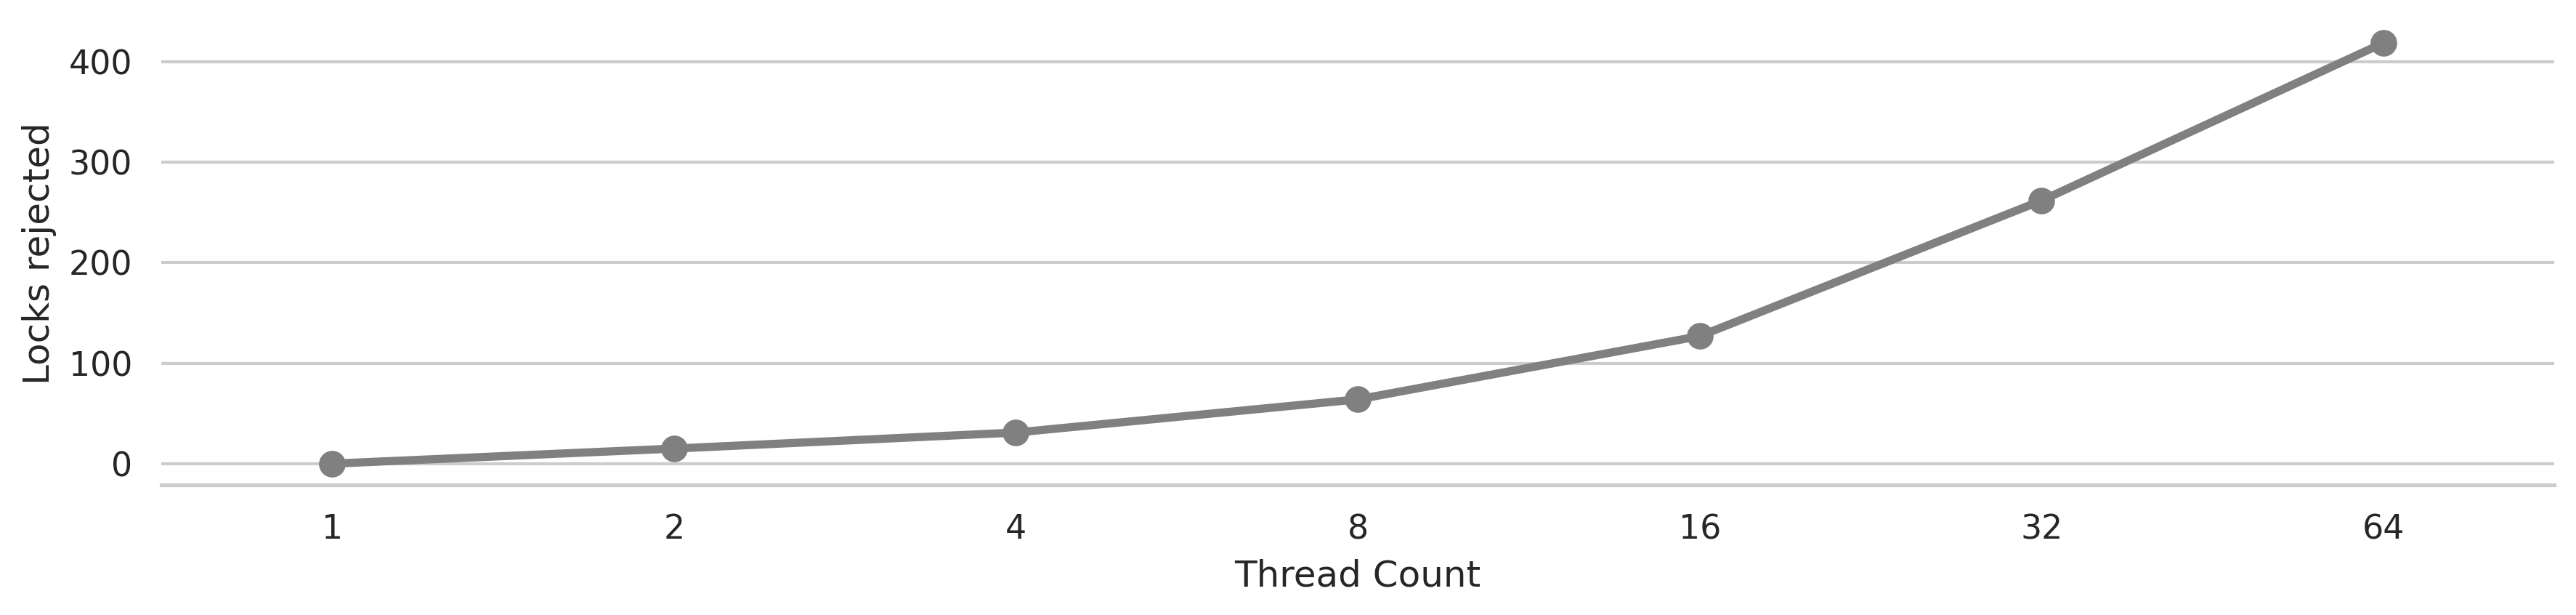
\includegraphics[width=.8\columnwidth]{PerformanceCharts/LockRejection.png}
% 	\caption{Locks rejected vs Thread Count}
% 	\label{lockRejection}
% \end{figure}

MGL techniques like DomLock, MID, FlexiGran and CALock are slower than coarse and medium grained locks. They are slow for reads and writes due to the presence of false subsumptions between grains causing spurious thread blocks. For structural modifications, DomLock, MID and FlexiGran spend time relabelling the hierarchy which is very expensive. 

CALock is faster than DomLock, MID and FlexiGran for reads and writes since it avoids false subsumptions (see Section \ref{benchmark:falseSubsumption}). For structual modifications, unlike DomLock, MID and FlexiGran, the relabelling can be parallelised if the lock grains do not overlap. When deleting vertices from the hierarchy (SM1), CALock does not require relabelling. 

% \begin{table*}
% 	\begin{tabular}{l|l|l|l|l|l|l}
% 		\textbf{Operation}	& \textbf{Coarse} 	& \textbf{Medium} 	& \textbf{DomLock} 	&\textbf{MID} 		& \textbf{FlexiGran} 	& \textbf{CALock} \\ \hline
% 		Q1 		& 35 		& 11 		& 560		& 1 		& 589 			& 3 	\\
% 		Q2 		& 43 		& 11 		& 1092 		& 3564 		& 1125 			& 11 	\\
% 		OP6 	& 32 		& 6 		& 560 		& 1 		& 6 			& 4 	\\
% 		OP7 	& 21 		& 1 		& 553 		& 1 		& 7 			& 5 	\\
% 		OP9	 	& 34 		& 3 		& 1 		& 1 		& 3 			& 3 	\\
% 		OP10 	& 31 		& 11 		& 1092 		& 1229 		& 1092 			& 15 	\\
% 		SM2 	& 1 		& 6 		& 556 		& 2427 		& 592 			& 2 	\\
% 		SM3 	& 1 		& 1 		& 560 		& 1266 		& 590 			& 7 	\\

% 	\end{tabular}
% \end{table*}

\begin{figure}
	\captionsetup{justification=centering}
	\centering
	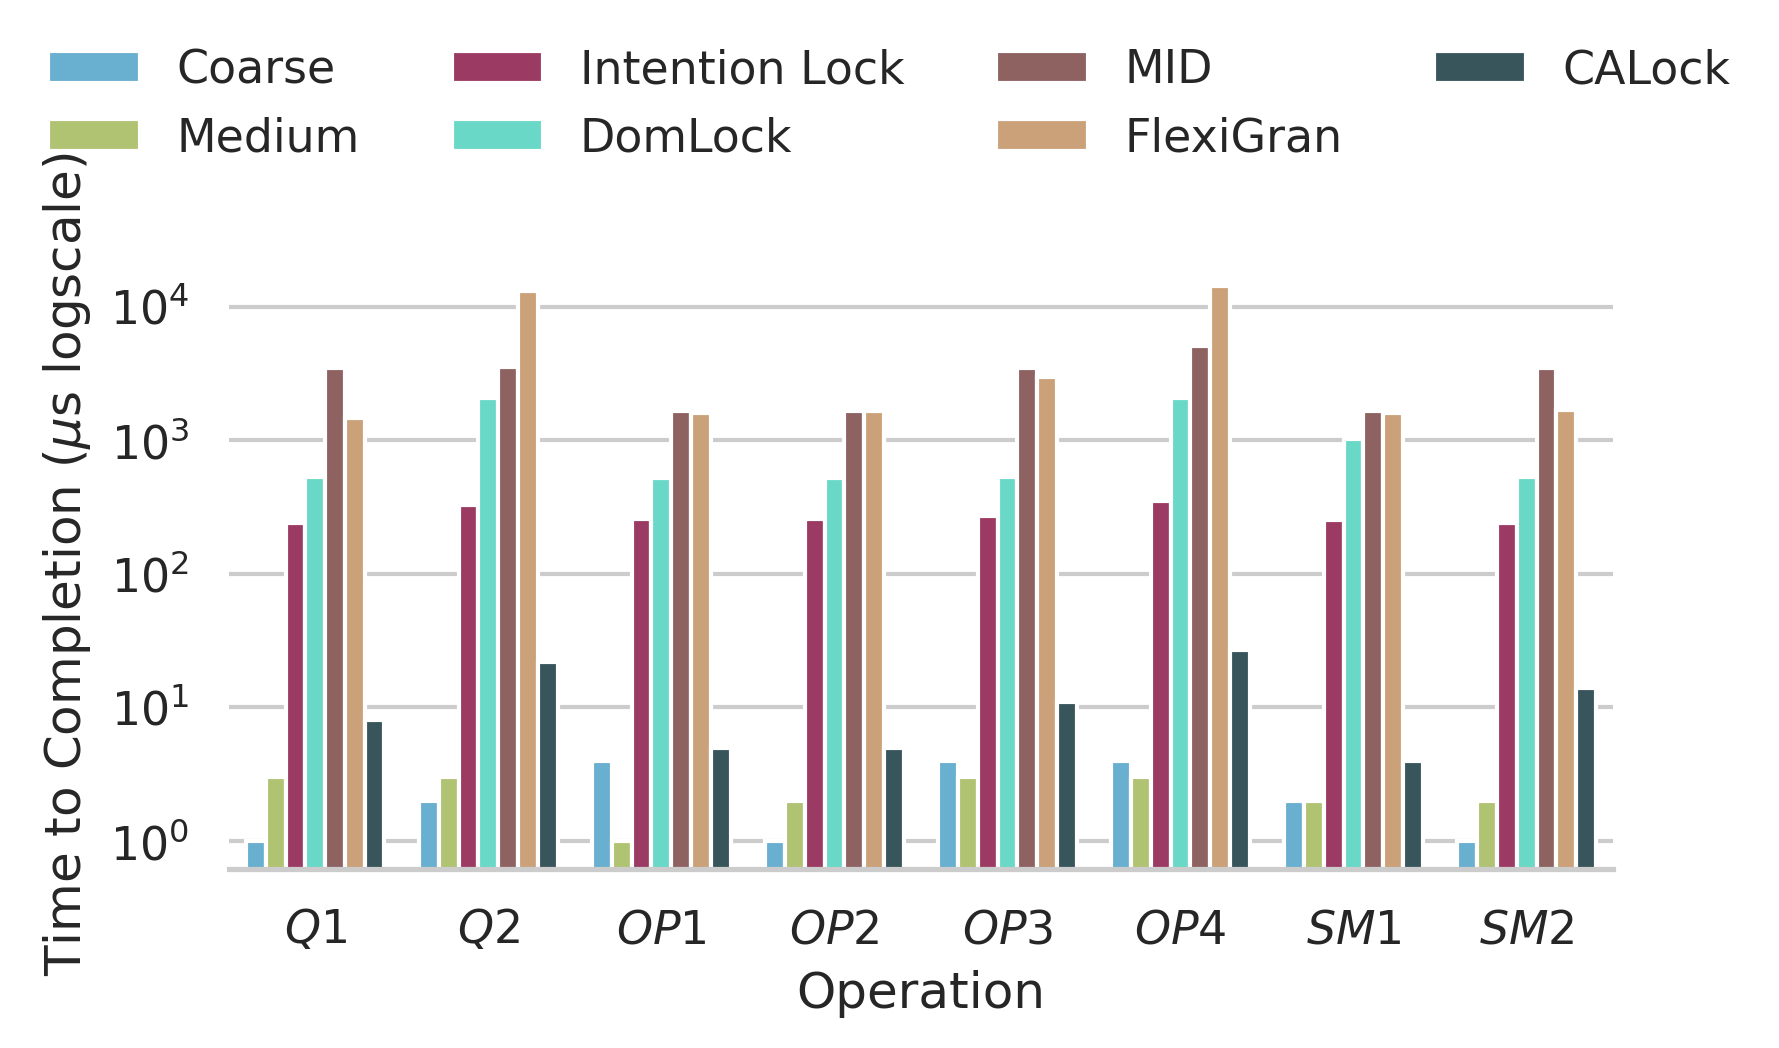
\includegraphics[width=\columnwidth]{figures/PerformanceCharts/TTC}
	\caption{Time to completion for different operations(lower is better). Deadlocks detected in Intentionlocks in grey.}
	\label{ttc}
\end{figure}


\section{Metadata management: bulk labelling and relabelling} \label
{benchmark:labellingAndRelabelling}
\subsection{Bulk labelling}

%\todo{Write text for preprocessing and explain the shortcuts that domlock takes to optimise interval assignment and how that leads to false subsumptions. }
We measure the time it takes to assign the labels to a graph when it is first created. 
This simulates loading data into a database.
Coarse-grain, medium-grain locks and intention locks do not need labelling. 
This time is measured for three different sizes of the STMBench7 graph. 
The results are shown in Figure \ref{initialLabelling}. 
We observe that DomLock is the fastest at preprocessing the hierarchy since a single depth-first-traversal is sufficient to compute the intervals. MID is slower than DomLock because it needs to compute two pairs of intervals for each vertex. One pair the intervals is computed by a depth-first traversal and another by a depth-first traversal on the mirror image of the graph. FlexiGran is faster than DomLock but slower than MID because of the additional level information that needs to be computed per vertex. 

CALock labels take the logest to preprocess since the labels are defined by a recursive breadth-first traversal with a fixpoint dependent on the number of paths to a vertex from the root.

\begin{figure}
	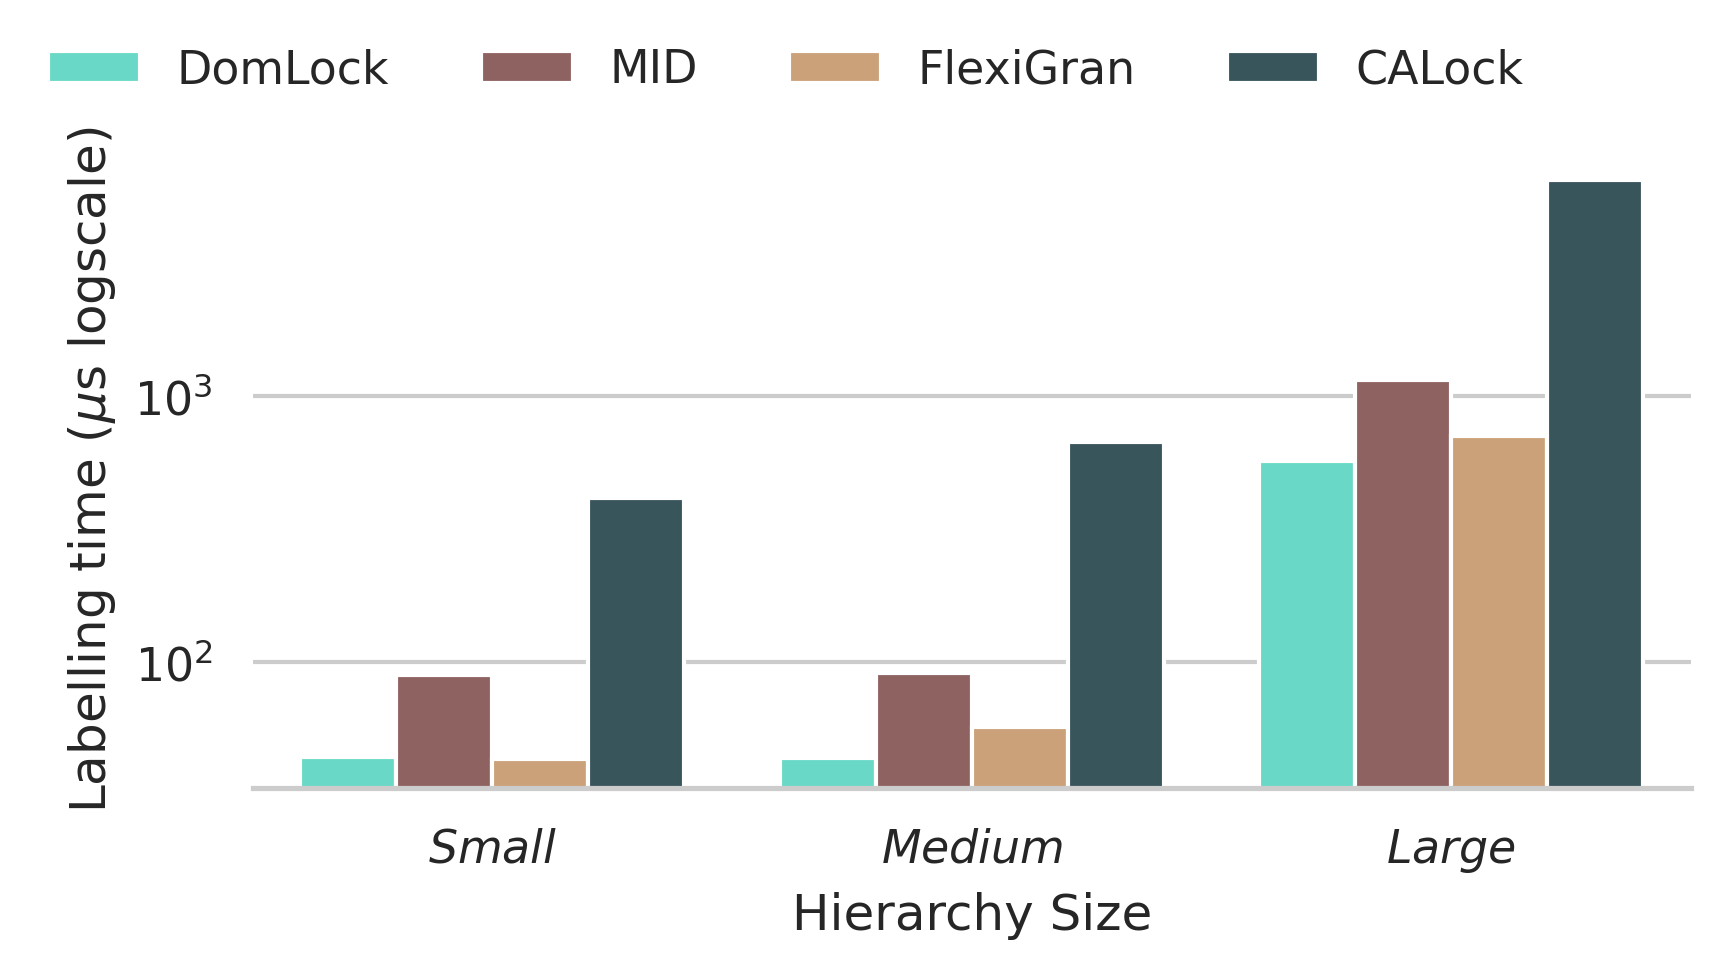
\includegraphics[width=\columnwidth]{figures/PerformanceCharts/InitialLabelling}
	\caption{Time to compute initial labels (lower is better)}
	\label{initialLabelling}
\end{figure}


\subsection{Relabelling}
Figure \ref{relabellingTime} shows the average time spent relabelling the graph per structural modification.
Both Coarse, medium grained locks and intention locks do not have additional metadata and hence do not require relabelling. 
In CALock, relabelling is significantly faster than DomLock, MID and FlexiGran. 
This is because in DomLock, MID and FlexiGran a structural modification anywhere in the graph changes the depth-first traversal order of several vertices of the graph. 
A change in this traversal order requires re-computing a lot of intervals which propagate to the root of the hierarchy. 
Since the root is involved in the relabeling, intervals are computed under a mutex on the graph which prevents parallel relabelling of disjoint subgraphs leading to poor performance of DomLock, MID and FlexiGran.  

In contrast, CALock relabels only the affected subgraphs directly affected by a structural modification. CALock labels always popagate away from the root towards the leaves and are computed under the lock that is acquired to perform the structural modification.
Thus, multiple grains can be locked, modified and relabelled in parallel. CALock is 2$\times$ faster at relabelling than DomLock, MID and FlexiGran.

%Both DomLock and CALock are faster with a higher number of threads because the STMBench graph slowly becomes less dense as a consequence of vertex deletions which in turn reduces the number of vertices that need to be relabelled.


%\todo{Change figure 9 With the updated results after the run is complete on grid5000}
\begin{figure}[ht]
	\captionsetup{justification=centering}
	\centering
	% \begin{subfigure}[b]{.325\textwidth}
		% \includegraphics[width=\columnwidth]{PerformanceCharts/ReadWithModificationsRelabelling}
		% \caption{R:90\%,W:9.9\%,SM:0.1\%}
	% \end{subfigure}
	% \begin{subfigure}[b]{.32\textwidth}
	% 	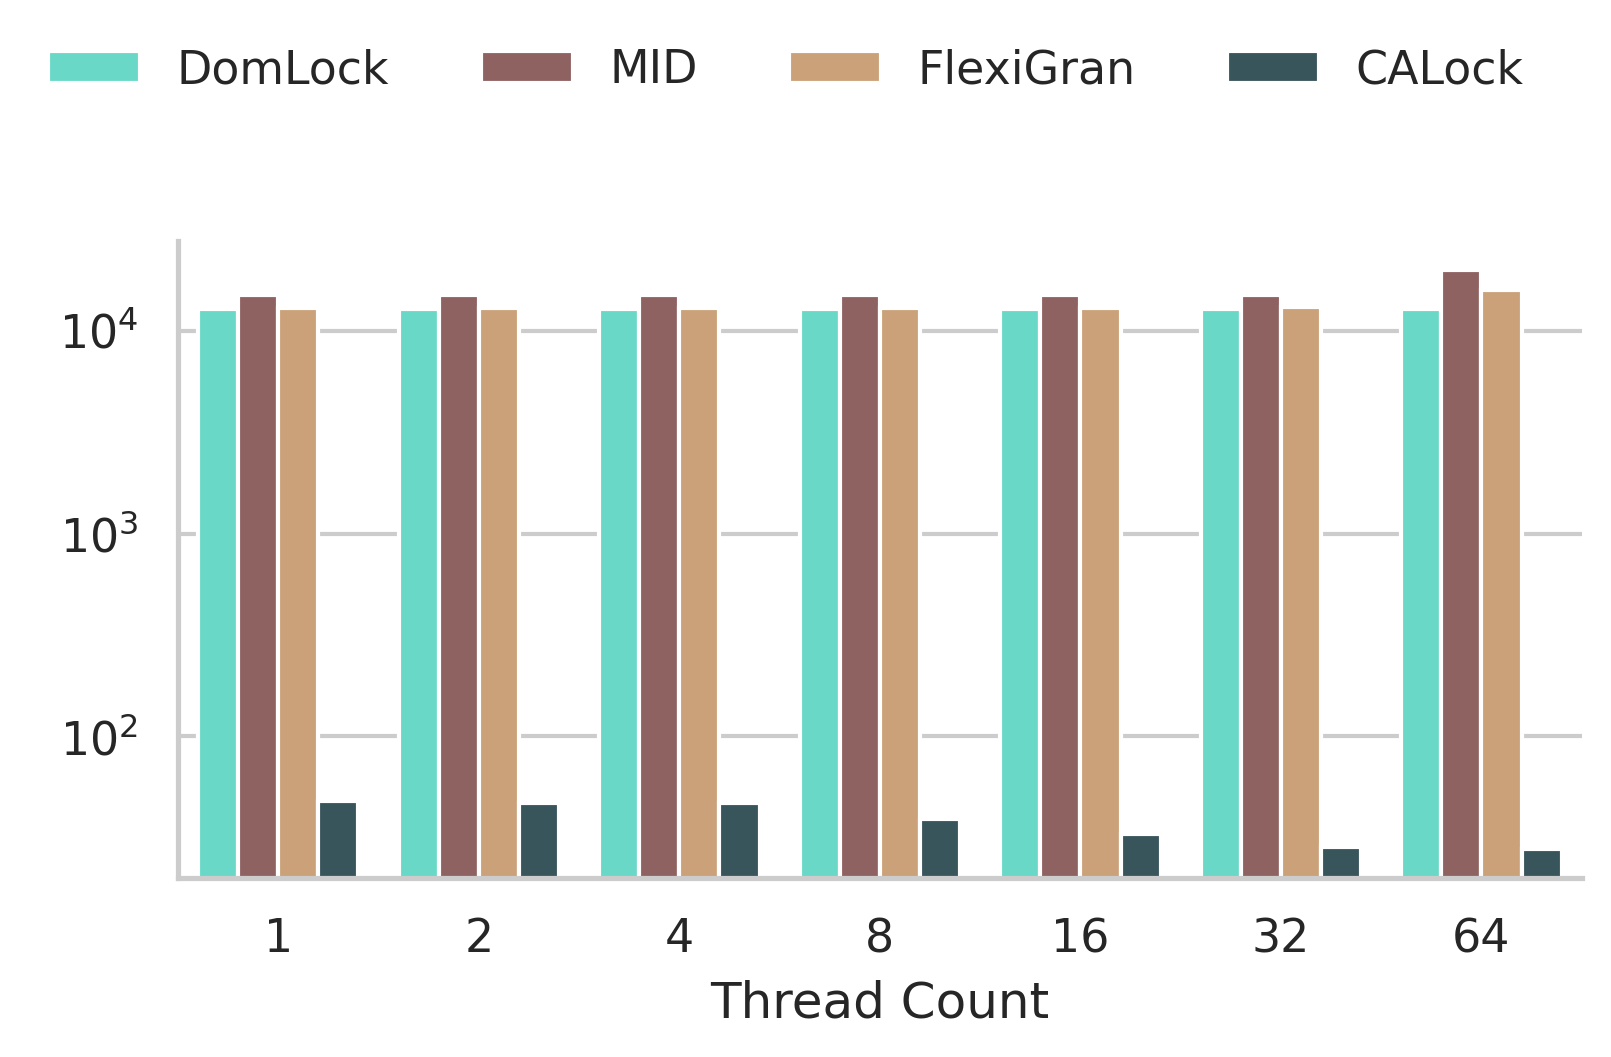
\includegraphics[width=\columnwidth]{PerformanceCharts/BalancedWithModificationsRelabelling}
	% 	\caption{R:60\%,W:39.6\%,SM:0.4\%}
	% \end{subfigure}
	% \begin{subfigure}[b]{.32\textwidth}
		\includegraphics[width=\columnwidth]{figures/PerformanceCharts/ReadWithModificationsRelabelling}
	% 	\caption{R:10\%,W:89.1\%,SM:0.9\%}
	% \end{subfigure}
	\caption{Time spent relabelling the graph per modification operation (lower is better)}
	\label{relabellingTime}
\end{figure}

%\todo{Make another benchmark to graph the relabelling time for different types of vertices similar to the subsumption benchmark in figure \ref{nodesLockedPerNodeType}}
\section{Metadata size in memory} \label{benchmark:metadatasize}
\begin{figure}[ht]
	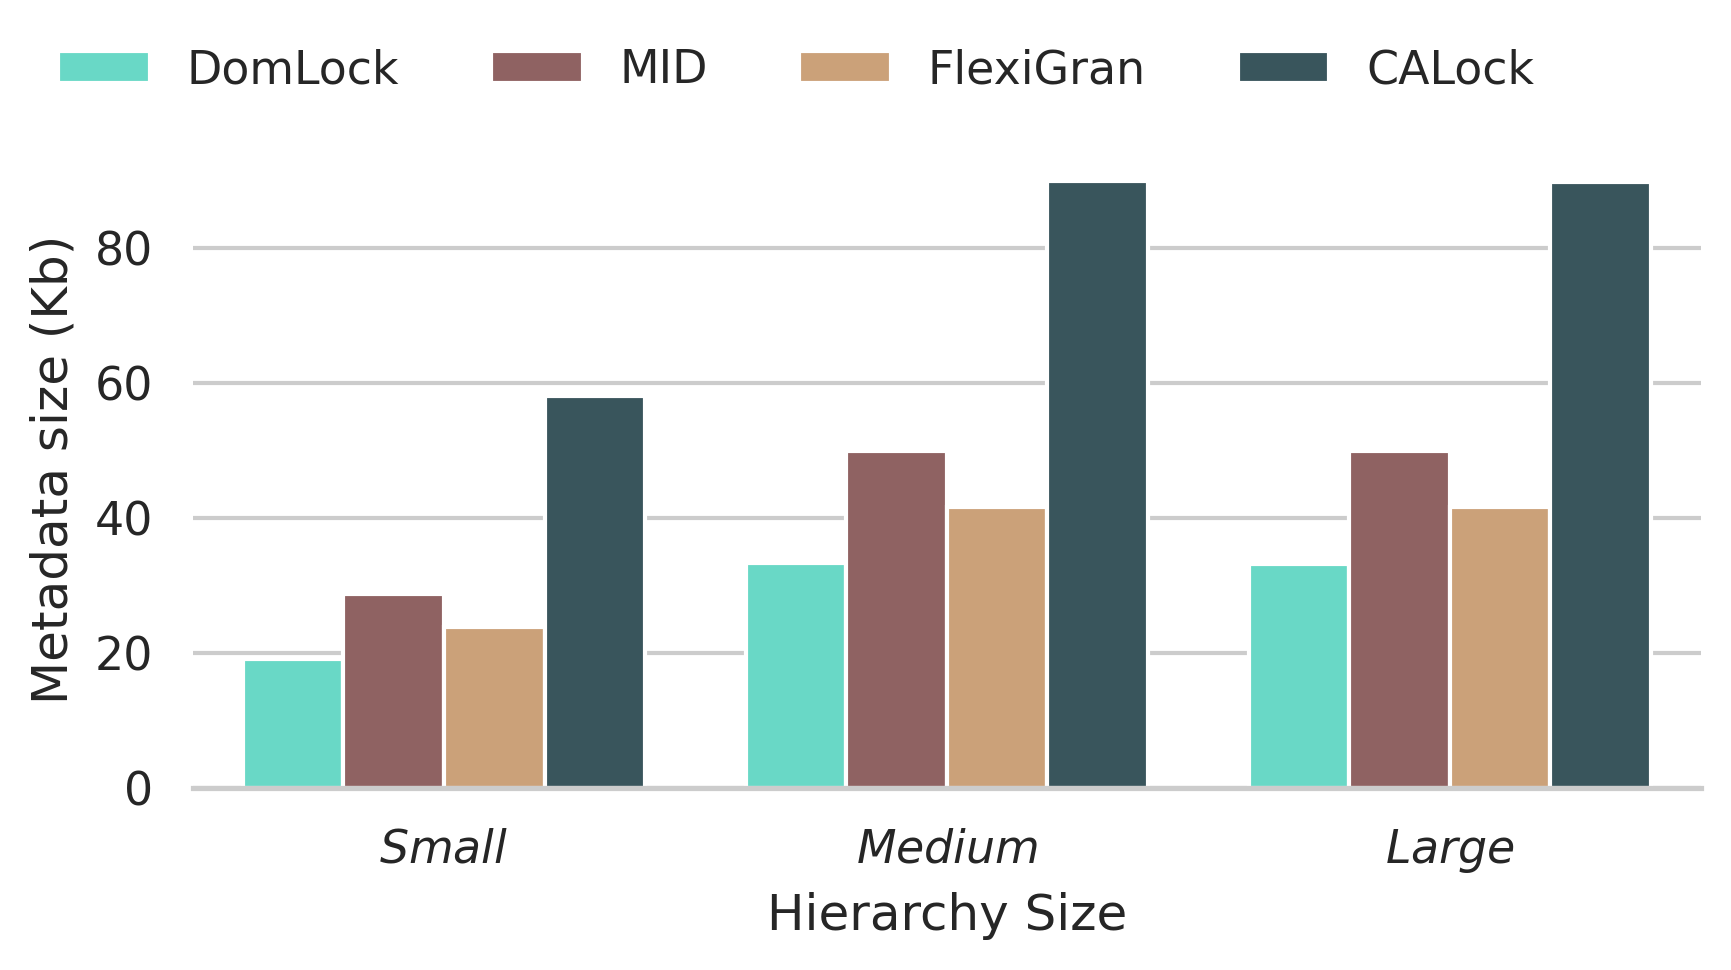
\includegraphics[width=\columnwidth]{figures/PerformanceCharts/LabelsMemorySize.png}
	\caption{Size of the metadata used for labelling}
	\label{metadataSize}
\end{figure}

All MGL techniques utilise metadata to identify the lock grains.
DomLock utilizes integer ranges as labels, which require less memory due to their compact representation. 
MID uses two pairs of integer ranges to represent the intervals of the vertices.
FlexiGran uses the DomLock intervals along with an integer to store the level of a vertex.
In contrast, CALock employs sets of vertex identifiers as labels, leading to a larger memory footprint.
As shown in Figure \ref{metadataSize}, CALock's metadata consumes approximately 1.5$\times$ more memory than DomLock, MID and FlexiGran.
In DomLock, MID and FlexiGran, regardless of the topology of the graph, the label at each vertex consists of integers.
This has low memory requirement however, the information about the exact topology of the graph is lost, leading to false subsumptions.
CALock labels, being sets, contain more information allowing for smaller grain sizes and prevent the problem of false subsumptions.


\section{Lock granularity and false subsumptions}\label{benchmark:falseSubsumption}

Locking a vertex in MGL implicitly also locks all other vertices present in the lock grain. 
To compare the grain size for them, we measure the number of targets implicitly locked for a guard vertex in the STMBench7 graph. 
Figure \ref{nodesLockedPerNodeType} compares the granularity of DomLock, MID, FlexiGran and CALock.

\begin{figure}
	\centering
	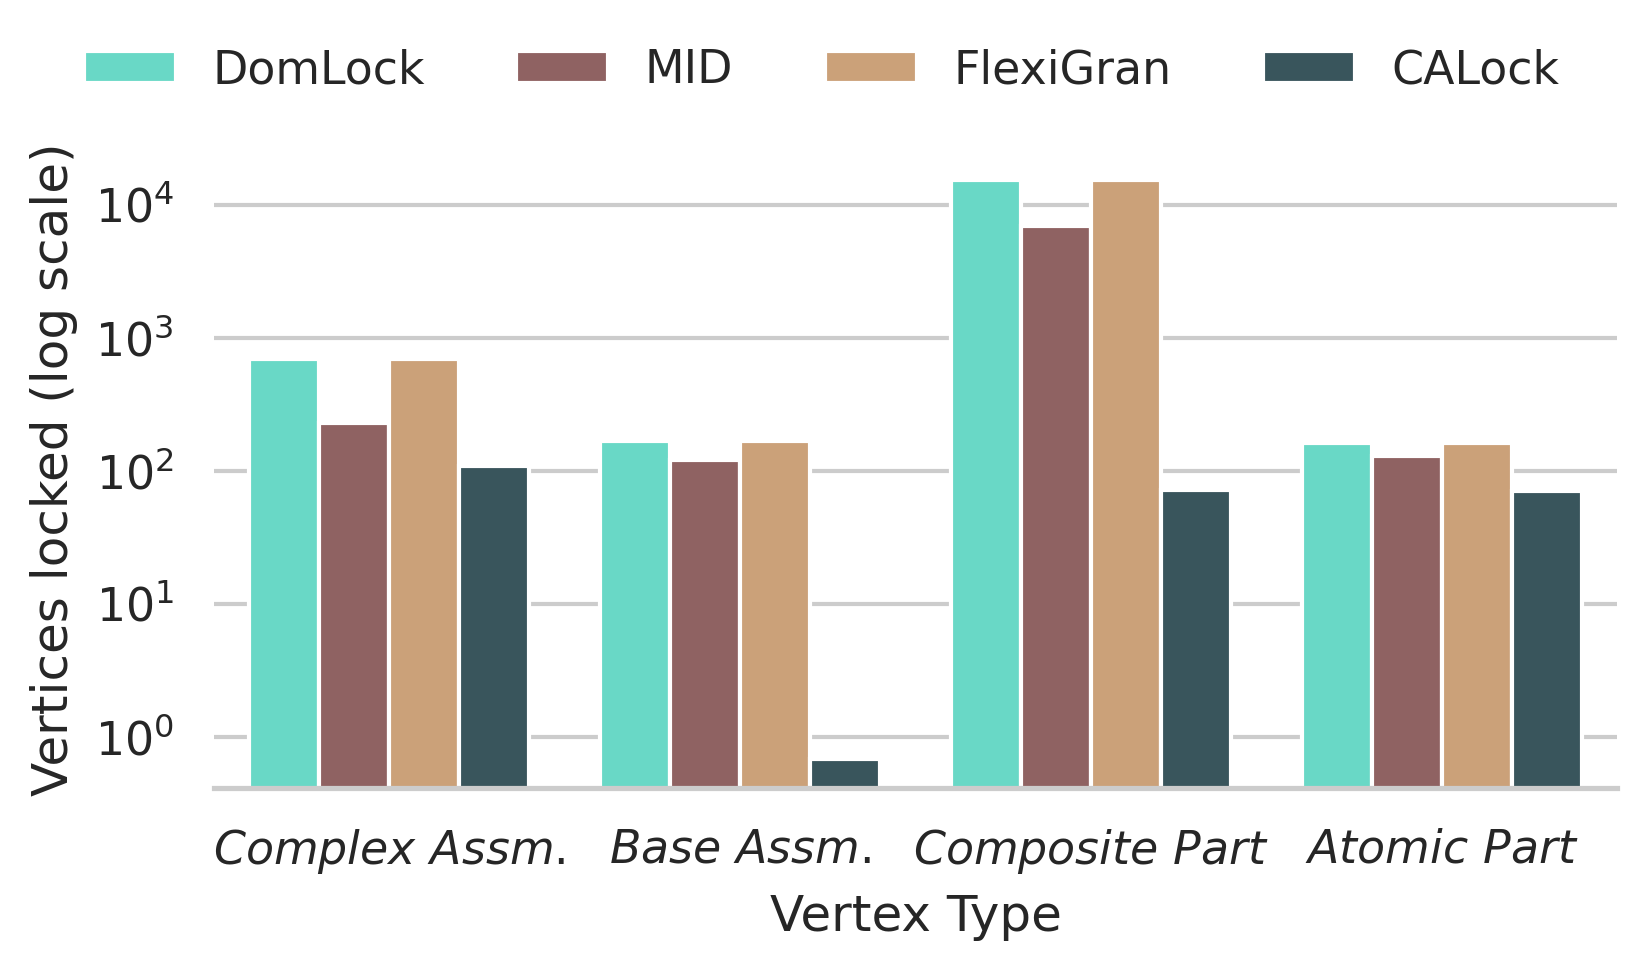
\includegraphics[width=\columnwidth]{figures/PerformanceCharts/ContainmentRatio}
	\caption{Vertices locked per vertex type (lower is better)}
	\label{nodesLockedPerNodeType}
\end{figure}

Locking an atomic part has almost the same effect for all techniques with CALock being marginally better and reducing grain sizes. 
This is because, in STMBench7, the atomic parts are strongly connected and locking a single vertex often causes the whole graph of atomic parts to be locked. 
When locking higher up in the graph, the effects vary. 
Locking a complex assembly is more expensive with intervals from DomLock, MID and FlexiGran because complex assemblies often share composite parts leading to large grains due to false subsumptions.
When locking base assemblies, with DomLock, MID and FlexiGran, multiple base assemblies are locked due to the one-to-many relationship between base assemblies and composite parts, again, owing to false subsumptions. 

The granularity of the lock and its effect on subsumption is highly dependent on the topology of the graph. 
False subsumptions aggravate the problem of large grains and lead to more grain overlaps between threads. 
The grain sizes of CALock are always smaller other locking techniques.


% \subsection{Effect of the lock request size} \label{benchmark:lockRequestSize}
% To study the effect of the size of a lock request on execution time, we set the synthetic benchmark to run a single thread that tries to lock consecutive leaf nodes. 
% A lock request with fewer vertices requires fewer set intersections to identify the LGCA for CALock and fewer integer comparisons to identify the lock interval for DomLock. 
% Figure \ref{requestSize} shows the results.

% \begin{figure}
% 	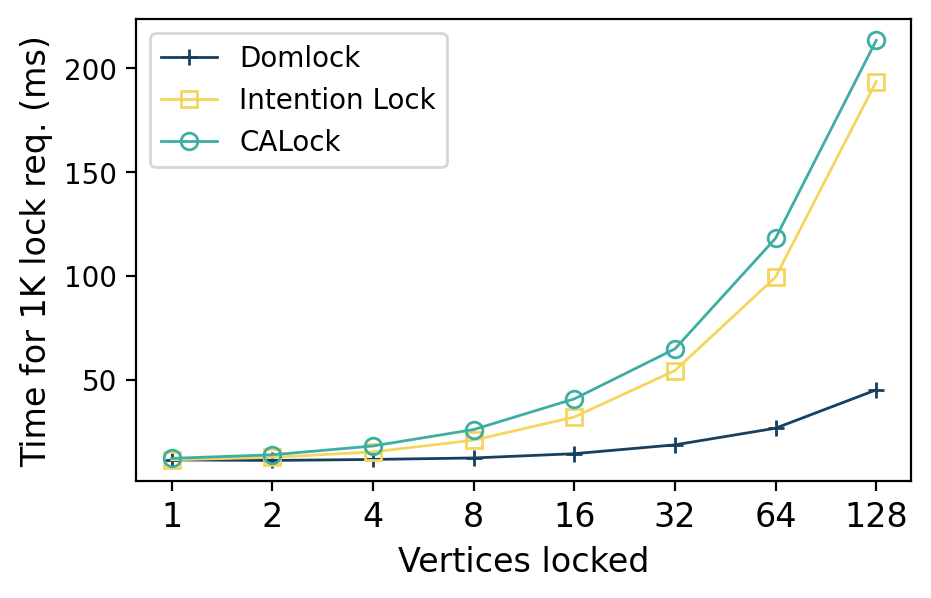
\includegraphics[width=.8\columnwidth]{PerformanceCharts/NodesPerLockRequestTree}
% 	\caption{Effect of lock request size (lower is better)}
% 	\label{requestSize}
% \end{figure}

% For small lock request sizes, the performance of Intention locks, DomLock and CALock is comparable. 
% Their performance diverges as the size of the request increases and DomLock performs best while CALock performs poorly. 
% Intention locks perform better than CALock because the paths to the lock guards are precomputed and stored as an index. 
% This eliminates the need for finding the guard vertex in the graph. 
% Trees have only one path to a vertex which reduces the the cost of placing intention tags along it. 
% The total cost of placing intention tags along the path is linear in the number of vertices being locked.
% %\todo{Complete this section with the details of how in graphs, CALock is better. Also run skewness benchmarks for Graphs. }

% The performance of CALock is poor when accessing several nodes because identifying the position of the lock in the graph requires a set intersection which has higher complexity compared to the integer comparison required for grain identification in DomLock. 
% This is especially bad for trees since the size of the label set for a vertex is equal to the depth of the vertex.


% \subsection{Effect of lock locality} \label{benchmar:lockLocality}

% \begin{figure}
% 	\includegraphics[width=.8\columnwidth]{PerformanceCharts/Skewness}
% 	\caption{Effect of lock locality (lower is better)}
% 	\label{skewedAccess}
% \end{figure}

% To study the effect of the access pattern of the vertices on performance, we configure the stress benchmark to run a fixed number of threads but restrict each thread to access a specific part of the tree for locking. 
% To achieve this, the leaf vertices of the tree are divided into disjoint buckets. A thread picks a bucket at random and creates a lock request for the vertices in that bucket.

% Figure \ref{skewedAccess} shows how this locality affects performance. 
% We observe that when the threads are allowed to lock anywhere in the graph i.e. the bucket size is 1, the probability of conflicts is higher. 
% Due to a large number of conflicts, threads wait longer for their locks and the overall performance degrades. 
% As the locality of access increases and threads are restricted to buckets, the number of conflicts decreases.
% This allows threads to make progress in parallel and leads to higher overall performance. 

\section{Overall locking performance}
Sections \ref{benchmark:PerOpLatency}, \ref{benchmark:labellingAndRelabelling}, \ref{benchmark:metadatasize} and \ref{benchmark:falseSubsumption} study individual parameters in isolation. Now, we study all of them together and evaluate their affects on overall performance of the locking techniques. For FlexiGran, the percentage of fine grained locks is set to 50\% as recommended by the authors in their paper \cite{FlexiGran2024}. In these set of benchmarks, we study both static and dynamic graphs in STMBench under the same workloads. 
Figures \ref{staticPerf} and \ref{dynamicPerf} show the throughput of different workloads on static graphs and dynamic graphs respectively. 
The charts in these figures are plotted with the number of concurrent threads on the x-axis and the throughput (op/s) or response time ($ns$) on the y-axis. 
Response time is measured from when the thread issues a lock request until the lock is granted.


\subsection{Static Graphs} \label{benchmark:StaticOverallPerf}

\begin{figure*}
	\centering
	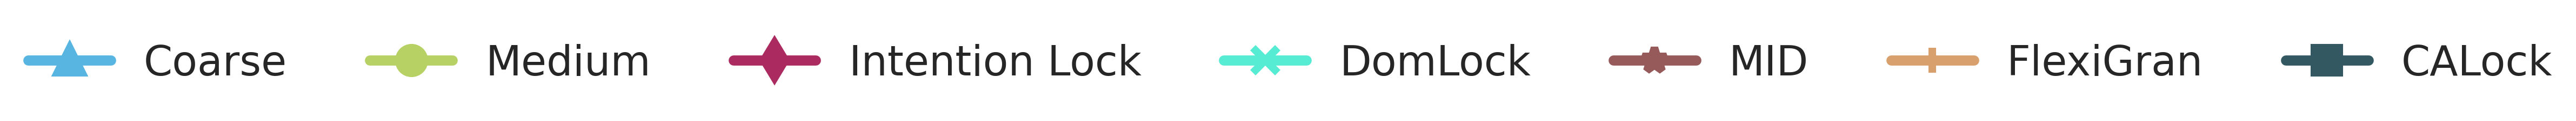
\includegraphics[width=.9\textwidth]{figures/PerformanceCharts/Legend}
\end{figure*}

\begin{figure*}[ht]
	\centering
	\captionsetup{justification=centering}
	\begin{subfigure}{.33\textwidth}
		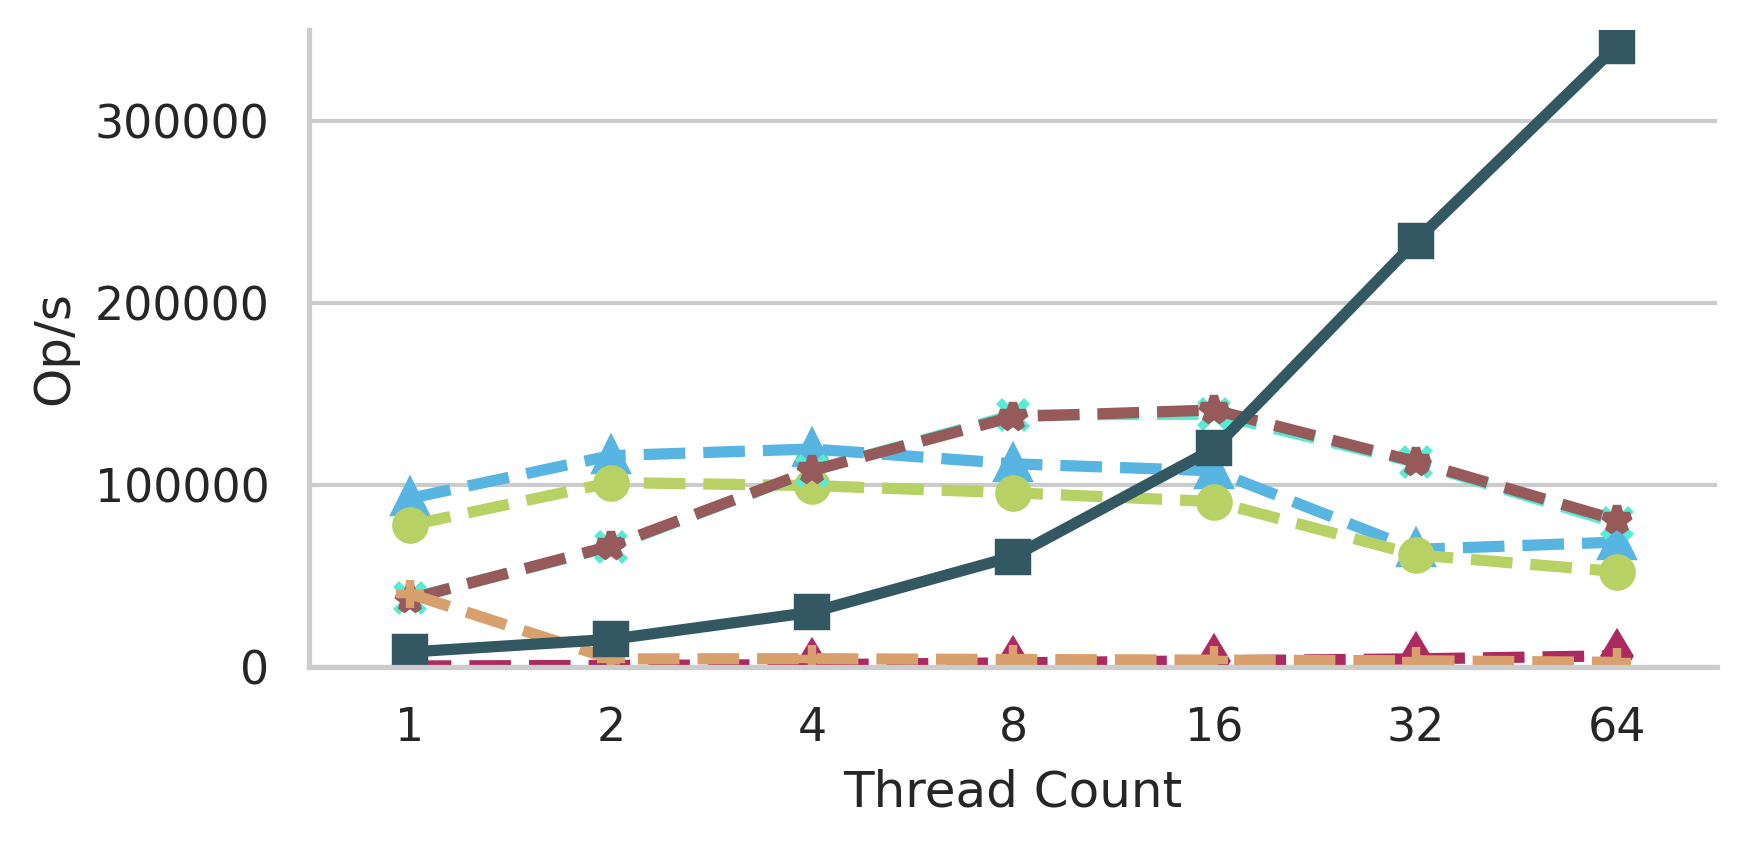
\includegraphics[width=\textwidth]{figures/PerformanceCharts/ReadWithoutModificationsThroughput}
		\caption{R:90\%,W:10\%}
		\label{rwm}
	\end{subfigure}
	\begin{subfigure}{.32\textwidth}
		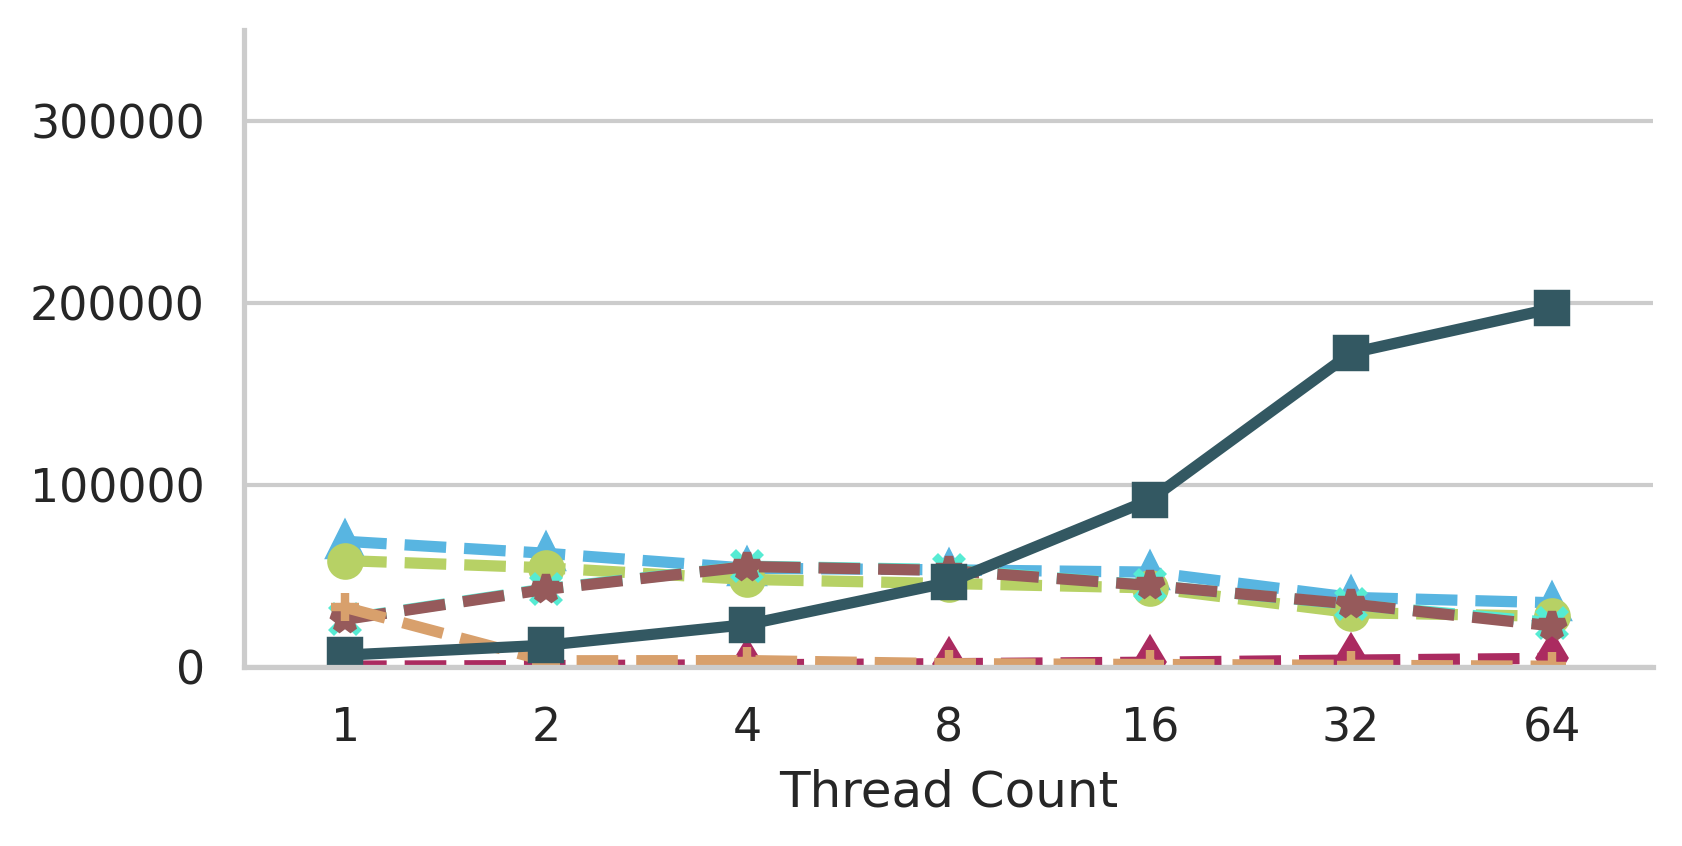
\includegraphics[width=\textwidth]{figures/PerformanceCharts/BalancedWithoutModificationsThroughput}
		\caption{R:60\%,W:40\%}
		\label{bwm}
	\end{subfigure}
	\begin{subfigure}{.32\textwidth}
		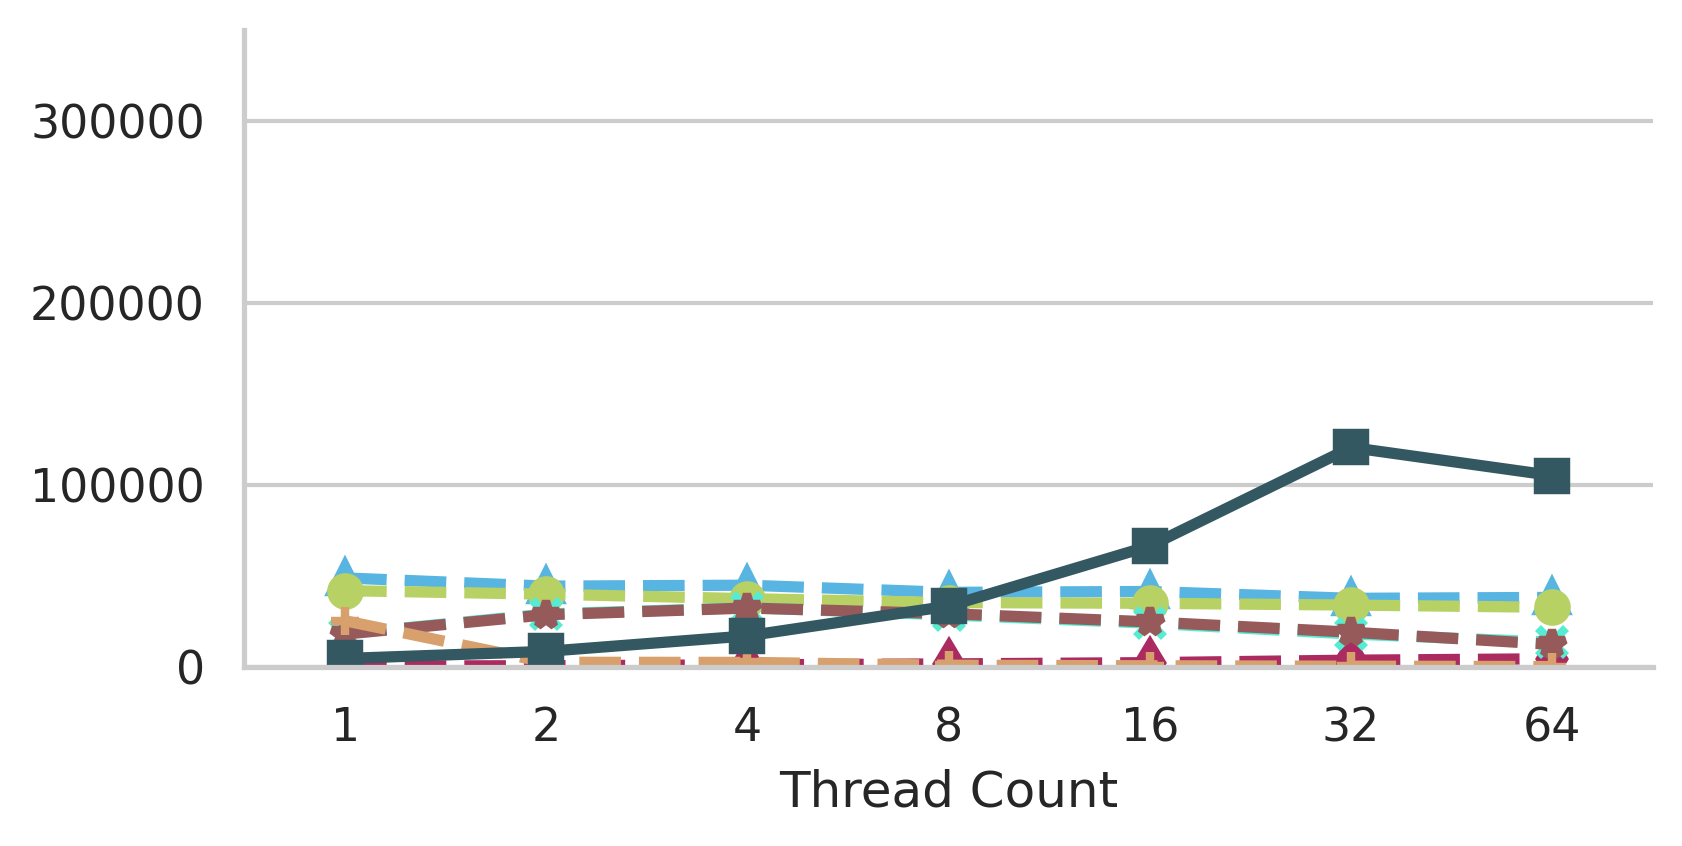
\includegraphics[width=\textwidth]{figures/PerformanceCharts/WriteWithoutModificationsThroughput}
		\caption{R:10\%,W:90\%}
		\label{wwm}
	\end{subfigure}
	\begin{subfigure}[b]{\textwidth}
		\caption*{\ref{rwm}, \ref{bwm}, \ref{wwm}: Throughput (higher is better)}
	\end{subfigure}


	\begin{subfigure}[b]{.33\textwidth}
		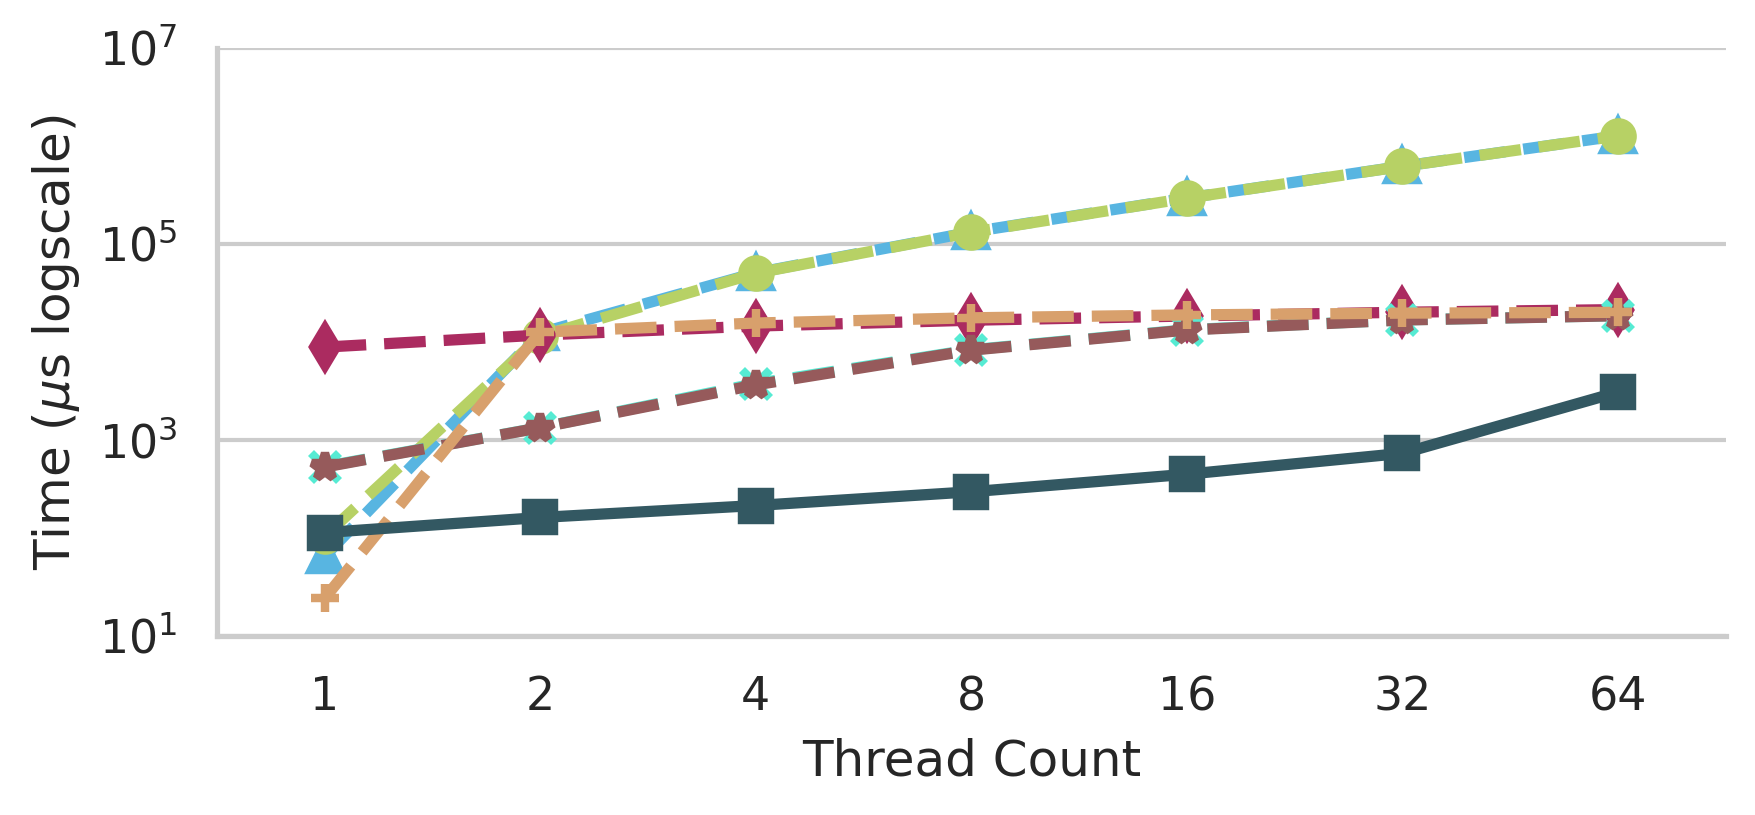
\includegraphics[width=\textwidth]{figures/PerformanceCharts/ReadWithoutModificationsIdleness}
		\caption{R:90\%,W:10\%}
		\label{irwm}
	\end{subfigure}
	\begin{subfigure}[b]{.32\textwidth}
		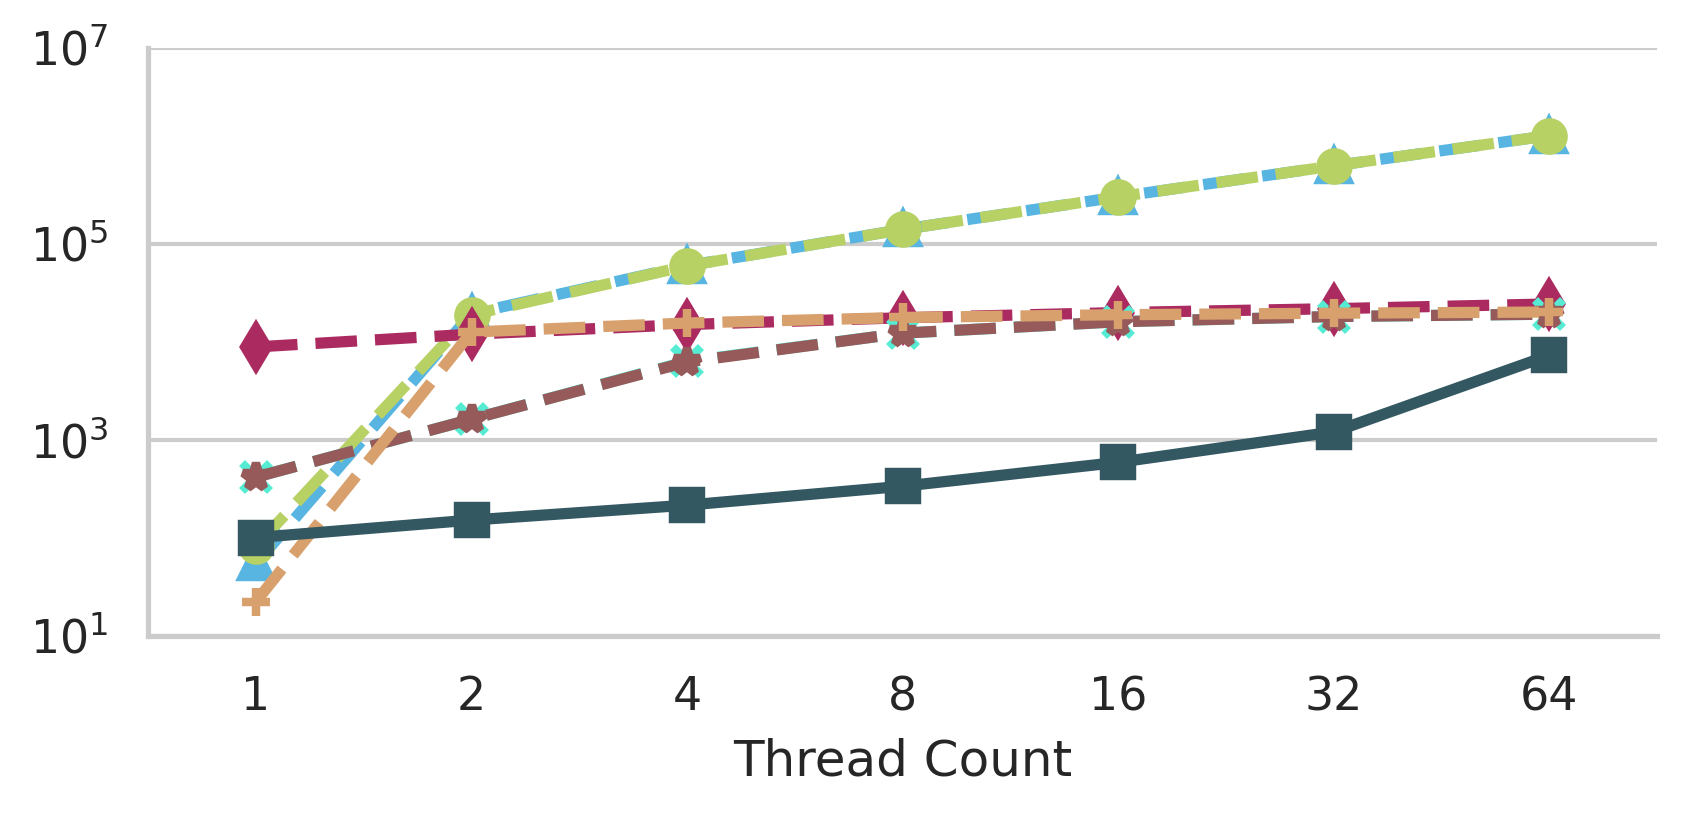
\includegraphics[width=\textwidth]{figures/PerformanceCharts/BalancedWithoutModificationsIdleness}
		\caption{R:60\%,W:40\%}
		\label{ibwm}
	\end{subfigure}
	\begin{subfigure}[b]{.32\textwidth}
		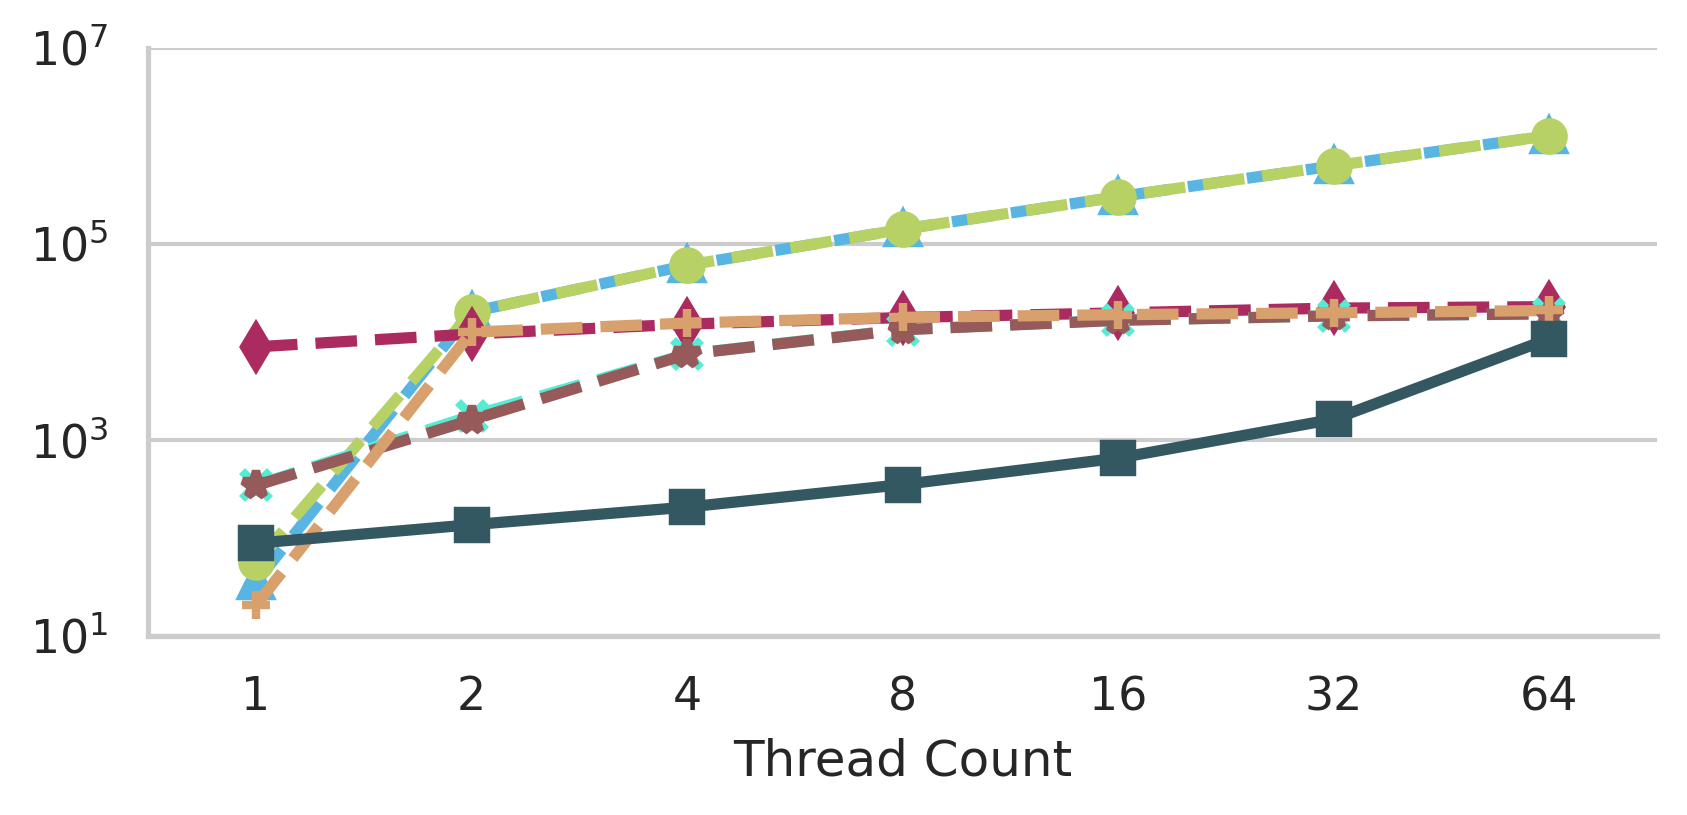
\includegraphics[width=\textwidth]{figures/PerformanceCharts/WriteWithoutModificationsIdleness}
		\caption{R:10\%,W:90\%}
		\label{iwwm}
	\end{subfigure}
	\begin{subfigure}[b]{\textwidth}
		\caption*{\ref{irwm}, \ref{ibwm}, \ref{iwwm}: Average time to grant lock request (lower is better)}
	\end{subfigure}



	\caption{Performance with different workload types on static graphs (R: reads, W: writes).}
	\label{staticPerf}
	\end{figure*}
Throughput figures \ref{rwm}, \ref{bwm} and \ref{wwm} show that coarse-grain and medium-grain locks perform the best for up to 4 concurrent threads due to the additional computation of the lock grain required for DomLock, MID, FlexiGran and CALock. Beyond 4 threads, MGL techniques give better throughput. However, the performance of DomLock and MID stagnates at 8 threads.

The graph in STMBench is irregular and has multiple paths leading to a vertex. Due to this, the lock grain sizes are uneven and DomLock, MID and Flexigran intervals often lead to false subsumptions which block a thread even when there is no conflict (see Section \ref{benchmark:falseSubsumption}). Intention locks often deadlock due to these irregular paths leading to poor performance(see Section\ref{ttc}). 

CALock successfully minimises the size of the lock grains and allows threads to lock disjoint grains in parallel achieving better scalability than DomLock, MID and FlexiGran.
We observe that CALock is 2x faster than DomLock for 32 threads and 4.5x faster than DomLock for 64 threads.

Observe that as the ratio of writes in a workload increases, the maximum throughput of any locking mechanism decreases because of inherent contention due to conflicts between write lock requests.


% Figure \ref{allReadPercentage} shows the trend of performance gain with an increasing ratio of reads for 32 concurrent readers/writers. 
% We see that as the proportion of reads increases, the performance of CALock and DomLock improves because reads can happen concurrently. However, DomLock is still slower than CALock because of false subsumptions that cause spurious thread blocking.

Response time figures \ref{irwm}, \ref{ibwm} and \ref{iwwm} plot the wait time per thread between coarse grain locks, medium grain locks, Intention locks,  DomLock, MID, FlexiGran and CALock.
Due to the static nature of coarse and medium lock grains as the number of threads increases, the response time also increases due to the increase in conflicts. For a single thread, coarse and medium locks are the fastest but with any amount of parallelism, their performance suffers. 

Between the MGL techniques, FlexiGran and Intention locks on average take the longest to grant a lock. With intention locks, this is because of the expensive traversals required to place intention tags on vertices. With FlexiGran, lock conflict detection is very expensive because of the coexistance of MGL and fine grained locks. DomLock and MID are faster than FlexiGran but remain significantly slower than CALock. 

In interval based MGL techniques like DomLock, MID and FlexiGran, once a lock request identifies an interval it wishes to lock, the thread traverses the hierarchy to find the lock guard, which is a vertex with the requested interval (resp. interval pair for MID). This traversal is especially expensive when locking deeper in the hierarchy. CALock on the other hand uses a set intersection to find the LGCA which is the ID of the vertex that needs to be locked. In doing so, CALock avoids traversals alltogether, giving faster response times for lock requests. 

The overall wait time increases with the number of concurrent threads because of an increase in the number of conflicts due to overlapping grains and the expensive conflict detection. For 64 threads, CALock is 6$\times$ faster than DomLock in a read-dominated load and 1.5$\times$ faster in a write-dominated load.



	% \begin{figure}
	% 	\captionsetup{justification=centering}
	% 	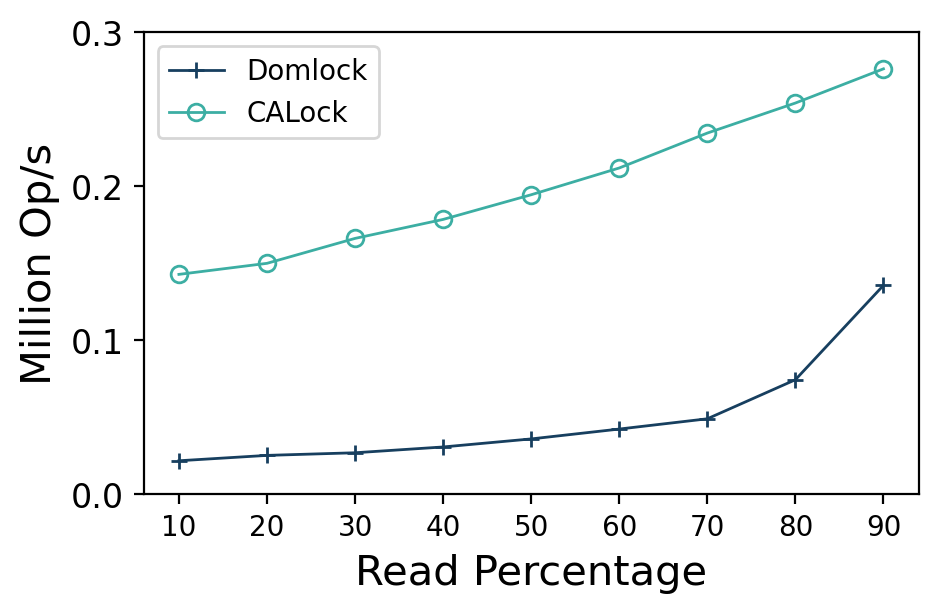
\includegraphics[width=0.8\columnwidth]{PerformanceCharts/ReadPercentageThroughput}
	% 	\caption{Comparing Domlock and CAlock with different read proportions on 32 threads (higher is better)}
	% 	\label{allReadPercentage}
	% \end{figure}


			% for which the improvement is slower but always remains better than DomLock overall.
			%\todo{Change the improves much faster line to something that says domlock is still bad.}


	



\subsection{Dynamic Graphs} \label{benchmark:DynamicOverallPerf}
\begin{figure*}[ht]
	\centering
	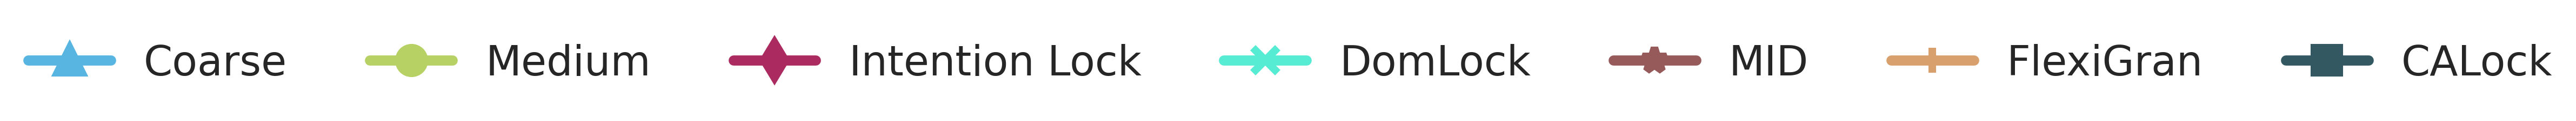
\includegraphics[width=.9\textwidth]{figures/PerformanceCharts/Legend}
\end{figure*}

\begin{figure*}[ht]
	\centering
	\captionsetup{justification=centering}
		\begin{subfigure}[b]{.33\textwidth}
			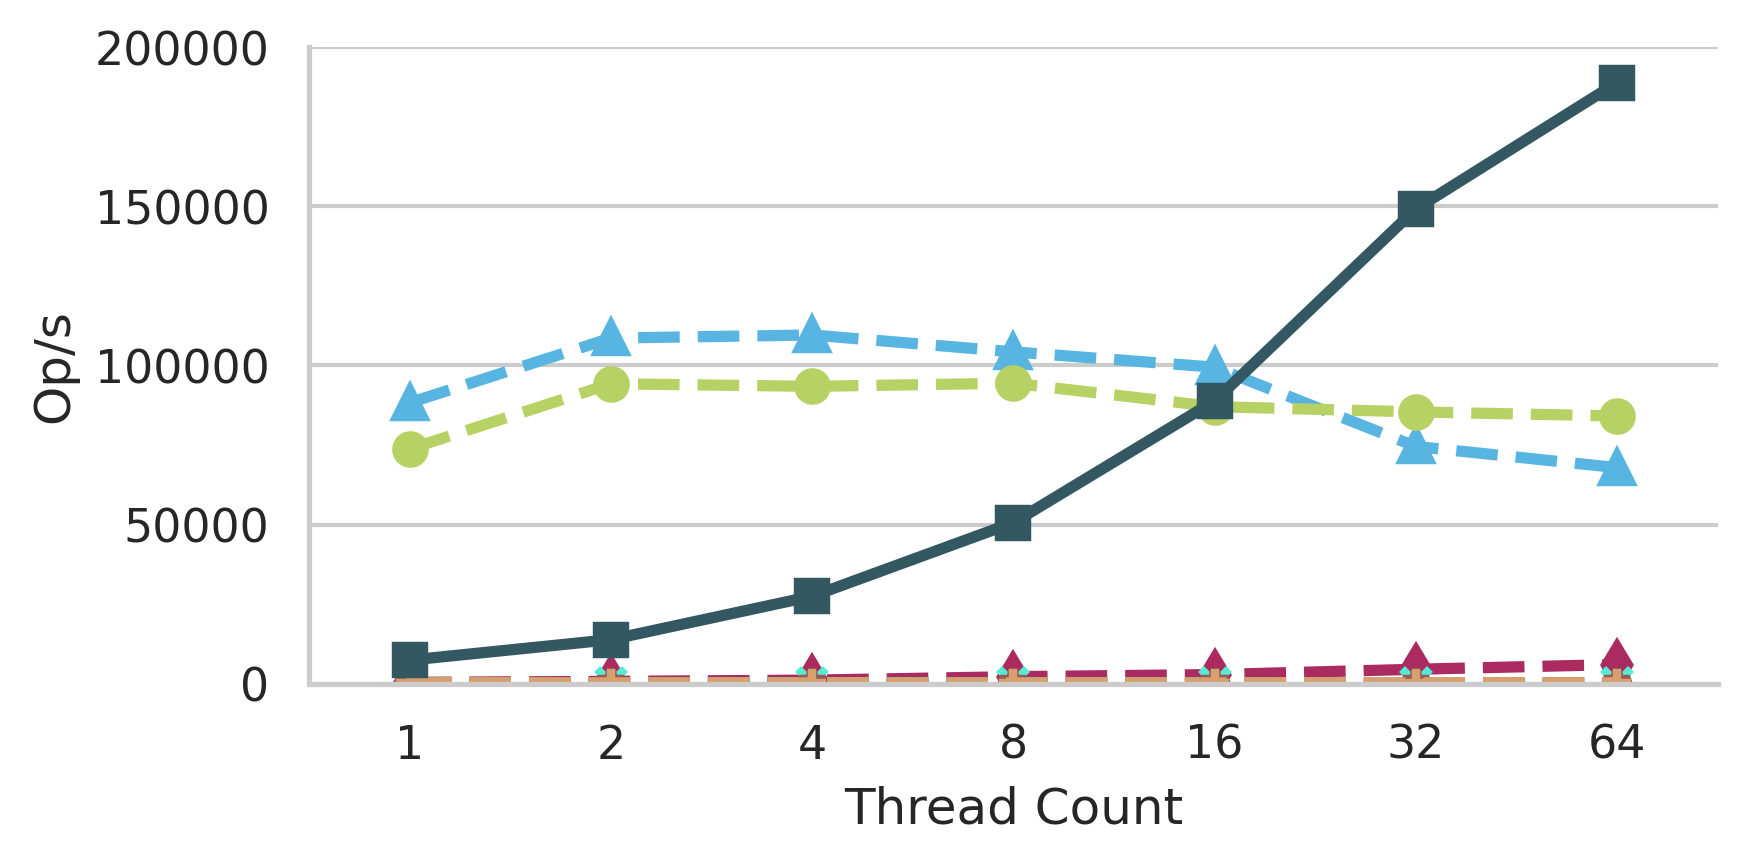
\includegraphics[width=\textwidth]{figures/PerformanceCharts/ReadWithModificationsThroughput}
			\caption{R:90\%,W:9.9\%,SM:0.1\%}
			\label{rm}
		\end{subfigure}
		\begin{subfigure}[b]{.325\textwidth}
			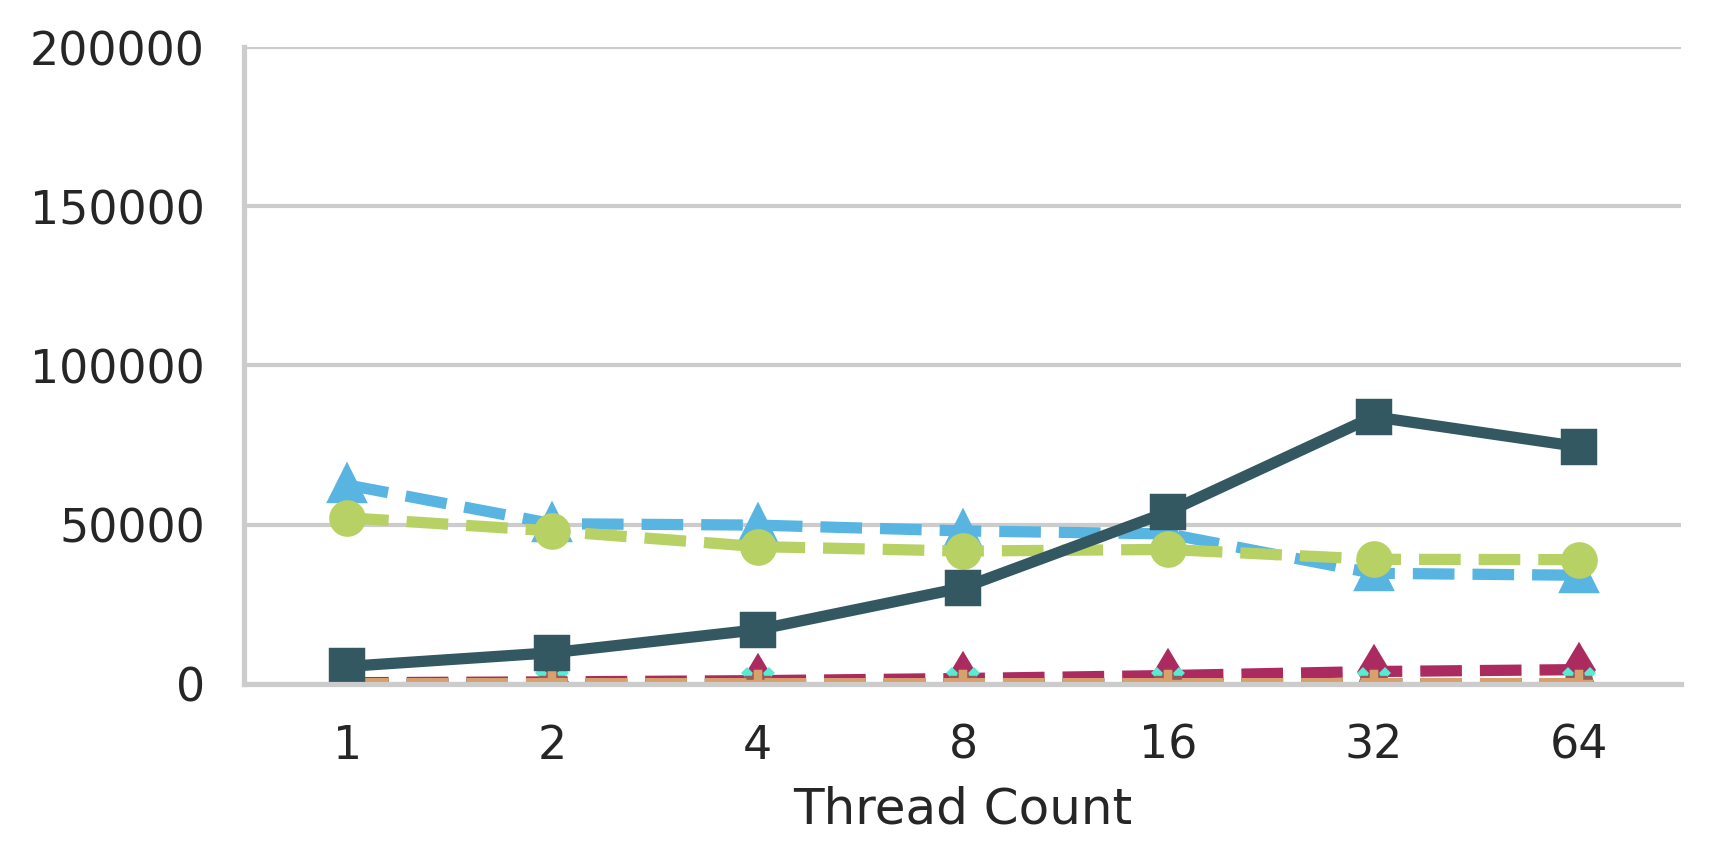
\includegraphics[width=\textwidth]{figures/PerformanceCharts/BalancedWithModificationsThroughput}
			\caption{R:60\%,W:39.6\%,SM:0.4\%}
			\label{bm}
		\end{subfigure}
		\begin{subfigure}[b]{.325\textwidth}
			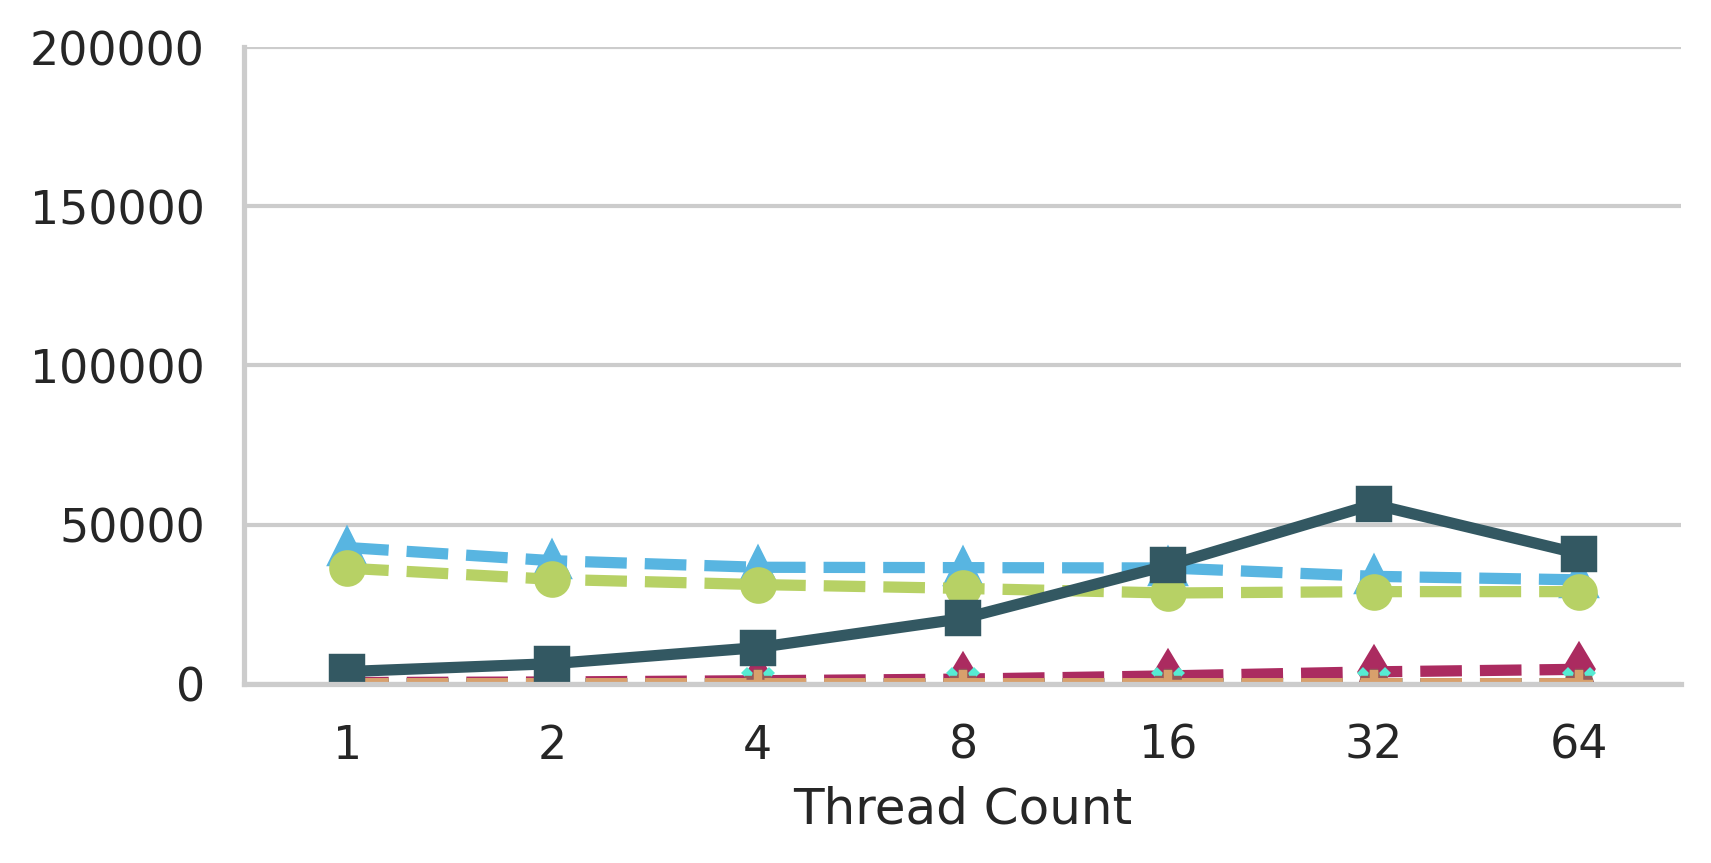
\includegraphics[width=\textwidth]{figures/PerformanceCharts/WriteWithModificationsThroughput}
			\caption{R:10\%,W:89.1\%,SM:0.9\%}
			\label{wm}
		\end{subfigure}
		\begin{subfigure}[b]{\textwidth}
			\caption*{\ref{rm}, \ref{bm}, \ref{wm} : Throughput (higher is better)}
		\end{subfigure}
	
	
	
		\begin{subfigure}[b]{.33\textwidth}
			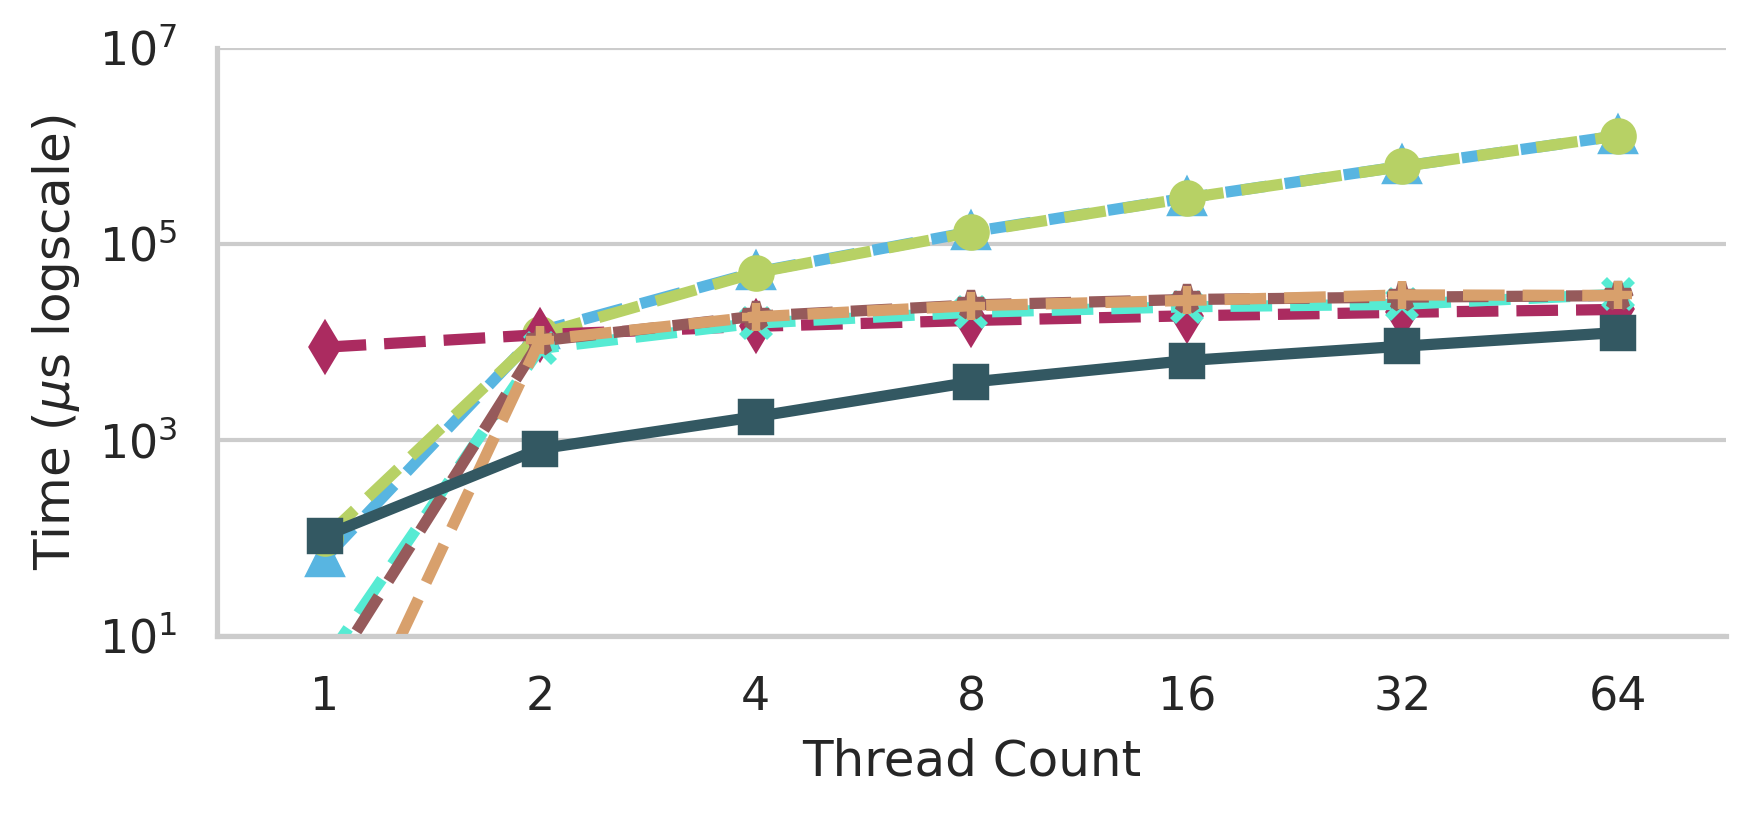
\includegraphics[width=\textwidth]{figures/PerformanceCharts/ReadWithModificationsIdleness}
			\caption{R:90\%,W:9.9,SM:0.1\%}
			\label{irm}
		\end{subfigure}
		\begin{subfigure}[b]{.325\textwidth}
			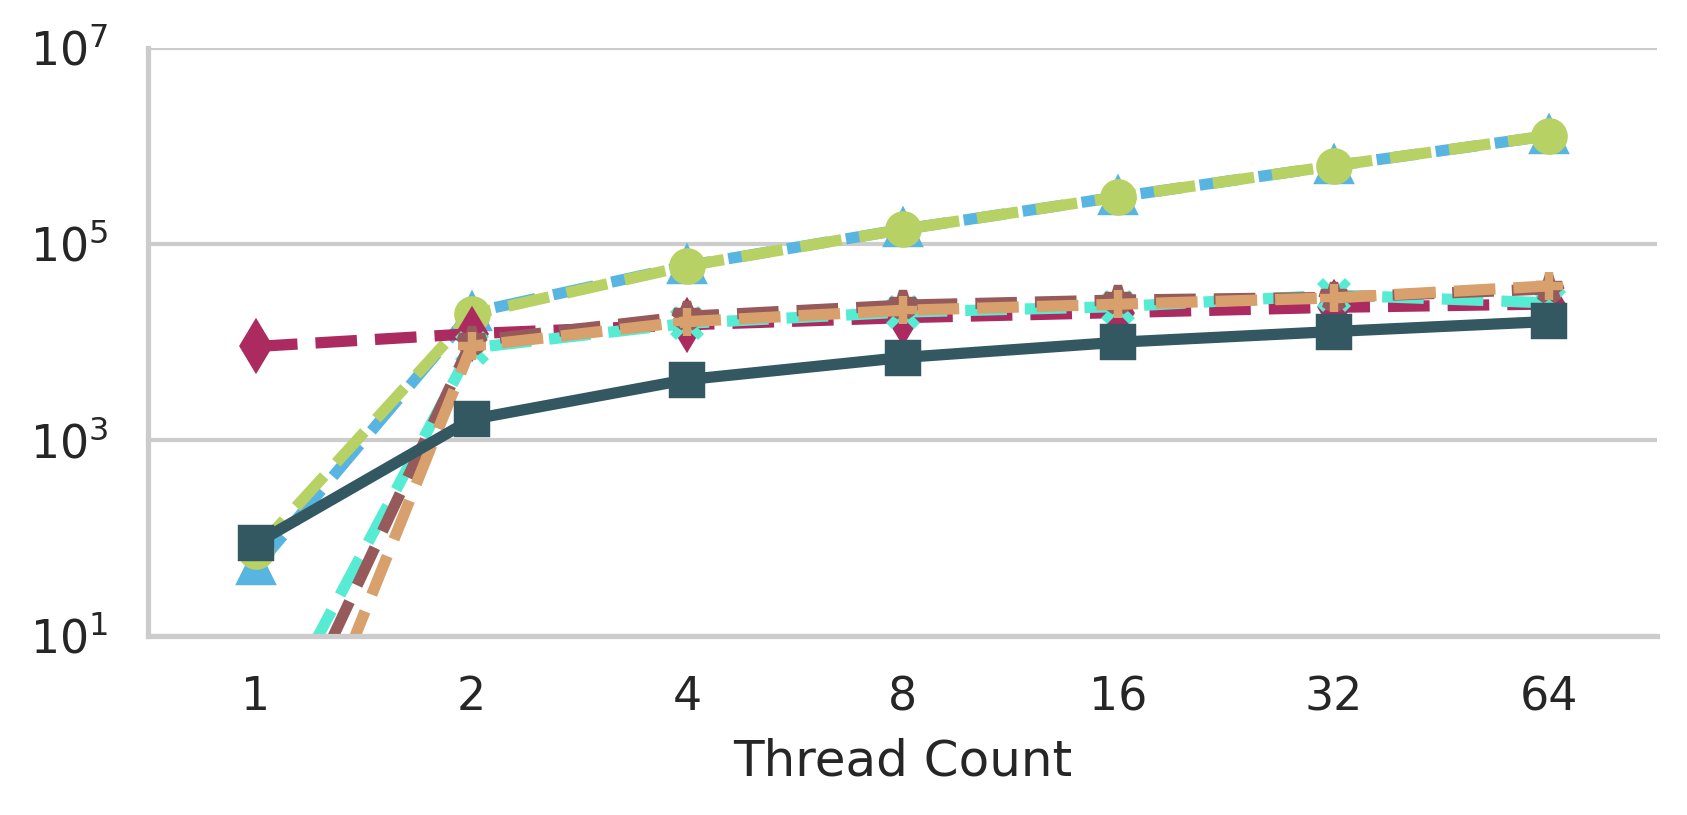
\includegraphics[width=\textwidth]{figures/PerformanceCharts/BalancedWithModificationsIdleness}
			\caption{R:60\%,W:39.6\%,SM:0.4\%}
			\label{ibm}
		\end{subfigure}
		\begin{subfigure}[b]{.325\textwidth}
			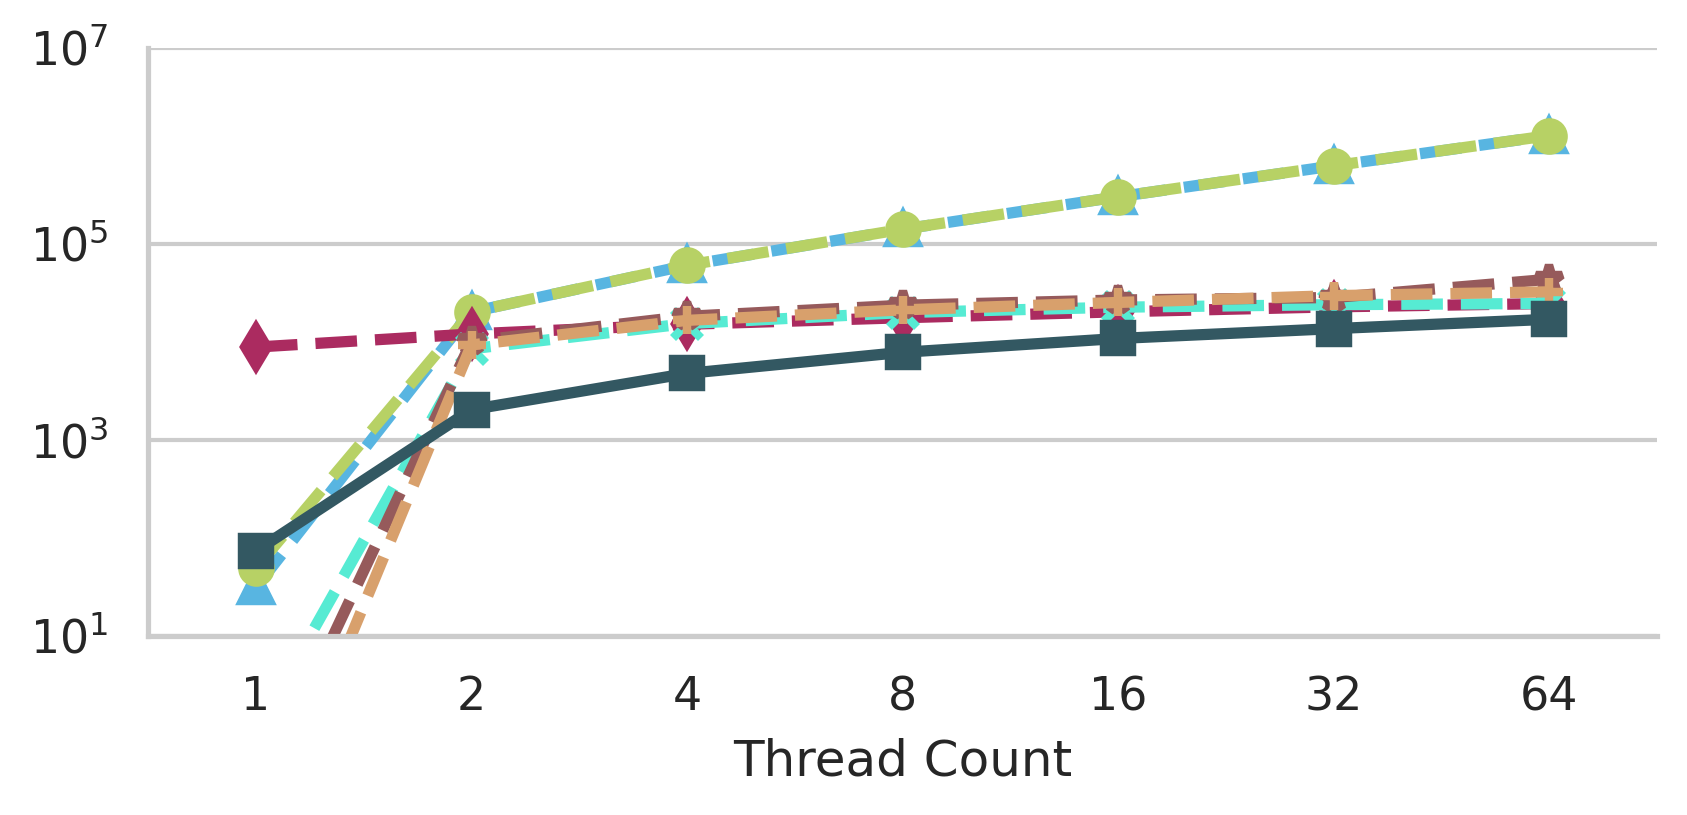
\includegraphics[width=\textwidth]{figures/PerformanceCharts/WriteWithModificationsIdleness}
			\caption{R:10\%,W:89.1\%,SM:0.9\%}
			\label{iwm}
		\end{subfigure}
		\begin{subfigure}[b]{\textwidth}
			\caption*{\ref{irm}, \ref{ibm}, \ref{iwm}: Average time to grant lock request  (lower is better)}
		\end{subfigure}
	
		\caption{Performance with different workload types on dynamic graphs  (R: reads, W: writes; SM: structural modifications).}
		\label{dynamicPerf}
	\end{figure*}
	
With structural modifications, the topology of the graph changes, triggering relabelling for MGL locking techniques like DomLock, MID, FlexiGran and CALock. 
Structural modifications happen under a mutex for coarse grain locks, medium grain locks, DomLock, MID and FlexiGran. 
Throughput figures \ref{rm}, \ref{bm} and \ref{wm} show the performance of locking algorithms under reads and writes that interleave with structural modifications leading to relabelling of the graph.
In these workloads, 10\% of the total writes are structural modifications.
In write-heavy workloads (Throughput figure \ref{wm}), structural modifications can be as high as 0.9\%. 
While in read-heavy workloads (Throughput figure \ref{rm}), they are as low as 0.1\%.
Even under a small load of structural modifications, we observe that coarse locks, medium locks do not scale well as the number of threads increases. Intention locks are no different. While structural modifications do not require any additional care in intention locks, the cost of placing intention tags on all vertices is very high.

DomLock, MID and FlexiGran perform significantly worse compared to other algorithms because along with the lack of parallelism, an additional relabelling step is required for each structural modification and this relabelling happens under a mutex.
This is shown in the curves in Throughput figures \ref{rm}, \ref{bm} and \ref{wm} for DomLock, MID and FlexiGran, which are relatively flat, indicating a lack of scalability. CALock can parallelize structural modifications and is 2x faster than coarse and medium-grained locks and about 8x faster than DomLock, MID and FlexiGran.

Response time for Intention locks is independent of the dynamicity of graph topology. However, response time for DomLock, MID and FlexiGran is longer in dynamic graphs compared to static graphs, as shown in Response time figures \ref{irm}, \ref{ibm} and \ref{iwm}.
Response time for CALock also increases for dynamic graphs when compared to static graphs but CALock remains faster than all other lock techniques for even the most contended workload.

	%Figures \ref{irm}, \ref{ibm} and \ref{iwm} plot the wait time per thread between DomLock and CALock in the presence of structural modifications. We observe that the wait time for DomLock requests is significantly higher. This is because the structural modification operations in DomLock require a mutex and block every other thread.


\section{Summary of experimental results}
\subsection{Discussion}
The initial labelling time is proportional to the size of the graph but in conjunction with other benchmark results, CALock is a better choice for runtime performance since the fast integer labels of DomLock, MID and FlexiGran require more expensive relabelling when the graph is modified by structural modification operations (see Section \ref{benchmark:labellingAndRelabelling}).

% Based on the results of the synthetic benchmarks, Intention locks are a good candidate for regular static graphs and DomLock might still be a better approach compared to CALock if relabelling is not required because the graph is static. However, CALock is a better choice for dynamic graphs since the total relabelling cost is lower (see Section \ref{benchmark:DynamicOverallPerf}).

\subsection{Summary}
With the results from the experiments using STMBench7 and microbenchmarks, we can derive the following conclusions.
\begin{itemize}
	\item Intention locks are the most expensive locking technique for any workload and are not suitable for irregular graphs.
	\item CALock is faster than DomLock, coarse-grain and medium-grain locks for any workload that involves more than 8 concurrent threads.

	\item In workloads with low contention on static graphs, CALock is at least 3$\times$ faster compared to any other locking technique.

	\item  In workloads with low contention and dynamic graphs, CALock is 1.5$\times$ faster than coarse-grain and medium-grain locks and 8x faster than DomLock, MID and FlexiGran.

	\item In workloads with high contention on static graphs, CALock is 2$\times$ faster than coarse-grained and medium-grained locks and 4$\times$ faster than DomLock, MID and FlexiGran
	\item In workloads with high contention and dynamic graphs, CALock performs as good as coarse-grain and medium-grain locks and 4$\times$ faster than DomLock, MID and FlexiGran
	\item CALock is an appropriate locking technique if the graph is irregular and dynamic (which makes DomLock, MID and FlexiGran unsuitable).
\end{itemize}
